\documentclass[twoside]{book}

% Packages required by doxygen
\usepackage{fixltx2e}
\usepackage{calc}
\usepackage{doxygen}
\usepackage[export]{adjustbox} % also loads graphicx
\usepackage{graphicx}
\usepackage[utf8]{inputenc}
\usepackage{makeidx}
\usepackage{multicol}
\usepackage{multirow}
\PassOptionsToPackage{warn}{textcomp}
\usepackage{textcomp}
\usepackage[nointegrals]{wasysym}
\usepackage[table]{xcolor}

% Font selection
\usepackage[T1]{fontenc}
\usepackage[scaled=.90]{helvet}
\usepackage{courier}
\usepackage{amssymb}
\usepackage{sectsty}
\renewcommand{\familydefault}{\sfdefault}
\allsectionsfont{%
  \fontseries{bc}\selectfont%
  \color{darkgray}%
}
\renewcommand{\DoxyLabelFont}{%
  \fontseries{bc}\selectfont%
  \color{darkgray}%
}
\newcommand{\+}{\discretionary{\mbox{\scriptsize$\hookleftarrow$}}{}{}}

% Page & text layout
\usepackage{geometry}
\geometry{%
  a4paper,%
  top=2.5cm,%
  bottom=2.5cm,%
  left=2.5cm,%
  right=2.5cm%
}
\tolerance=750
\hfuzz=15pt
\hbadness=750
\setlength{\emergencystretch}{15pt}
\setlength{\parindent}{0cm}
\setlength{\parskip}{3ex plus 2ex minus 2ex}
\makeatletter
\renewcommand{\paragraph}{%
  \@startsection{paragraph}{4}{0ex}{-1.0ex}{1.0ex}{%
    \normalfont\normalsize\bfseries\SS@parafont%
  }%
}
\renewcommand{\subparagraph}{%
  \@startsection{subparagraph}{5}{0ex}{-1.0ex}{1.0ex}{%
    \normalfont\normalsize\bfseries\SS@subparafont%
  }%
}
\makeatother

% Headers & footers
\usepackage{fancyhdr}
\pagestyle{fancyplain}
\fancyhead[LE]{\fancyplain{}{\bfseries\thepage}}
\fancyhead[CE]{\fancyplain{}{}}
\fancyhead[RE]{\fancyplain{}{\bfseries\leftmark}}
\fancyhead[LO]{\fancyplain{}{\bfseries\rightmark}}
\fancyhead[CO]{\fancyplain{}{}}
\fancyhead[RO]{\fancyplain{}{\bfseries\thepage}}
\fancyfoot[LE]{\fancyplain{}{}}
\fancyfoot[CE]{\fancyplain{}{}}
\fancyfoot[RE]{\fancyplain{}{\bfseries\scriptsize Generated by Doxygen }}
\fancyfoot[LO]{\fancyplain{}{\bfseries\scriptsize Generated by Doxygen }}
\fancyfoot[CO]{\fancyplain{}{}}
\fancyfoot[RO]{\fancyplain{}{}}
\renewcommand{\footrulewidth}{0.4pt}
\renewcommand{\chaptermark}[1]{%
  \markboth{#1}{}%
}
\renewcommand{\sectionmark}[1]{%
  \markright{\thesection\ #1}%
}

% Indices & bibliography
\usepackage{natbib}
\usepackage[titles]{tocloft}
\setcounter{tocdepth}{3}
\setcounter{secnumdepth}{5}
\makeindex

% Hyperlinks (required, but should be loaded last)
\usepackage{ifpdf}
\ifpdf
  \usepackage[pdftex,pagebackref=true]{hyperref}
\else
  \usepackage[ps2pdf,pagebackref=true]{hyperref}
\fi
\hypersetup{%
  colorlinks=true,%
  linkcolor=blue,%
  citecolor=blue,%
  unicode%
}

% Custom commands
\newcommand{\clearemptydoublepage}{%
  \newpage{\pagestyle{empty}\cleardoublepage}%
}

\usepackage{caption}
\captionsetup{labelsep=space,justification=centering,font={bf},singlelinecheck=off,skip=4pt,position=top}

%===== C O N T E N T S =====

\begin{document}

% Titlepage & ToC
\hypersetup{pageanchor=false,
             bookmarksnumbered=true,
             pdfencoding=unicode
            }
\pagenumbering{alph}
\begin{titlepage}
\vspace*{7cm}
\begin{center}%
{\Large P2\+P-\/contract }\\
\vspace*{1cm}
{\large Generated by Doxygen 1.8.14}\\
\end{center}
\end{titlepage}
\clearemptydoublepage
\pagenumbering{roman}
\tableofcontents
\clearemptydoublepage
\pagenumbering{arabic}
\hypersetup{pageanchor=true}

%--- Begin generated contents ---
\chapter{Main Page}
\label{index}\hypertarget{index}{}Протокол U\+N\+I\+C\+O\+RE предлагает инновационный механизм перераспределения ценности в замкнутой цифровой экономической системе на основе математического алгоритма точного финансового планирования \char`\"{}Двойная Спираль\char`\"{}.


\begin{DoxyItemize}
\item Исполняется в любой сетевой операционной системе типа E\+OS.
\item Генерирует теоретически неограниченную прибыль при фиксированных рисках и абсолютном финансовом балансе в любой момент.
\item Предоставляет инновационную бизнес-\/модель, основанную на энергии внимания и добровольных пожертвованиях людей.
\end{DoxyItemize}\hypertarget{index_purpose_sec}{}\section{Назначение}\label{index_purpose_sec}
Протокол предназначен для запуска и обслуживания цифровых экономических систем \char`\"{}Двойная Спираль\char`\"{} во множестве различных конфигураций с целью увеличения качества жизни участников за счёт ускоренного движения финансовых потоков между ними. \hypertarget{index_install_sec}{}\section{Клуб разработчиков}\label{index_install_sec}
\href{https://unicode.club}{\tt https\+://unicode.\+club}\hypertarget{index_licension_sec}{}\section{Лицензия}\label{index_licension_sec}
M\+IT 
\chapter{Hierarchical Index}
\section{Class Hierarchy}
This inheritance list is sorted roughly, but not completely, alphabetically\+:\begin{DoxyCompactList}
\item \contentsline{section}{ahosts}{\pageref{structahosts}}{}
\item \contentsline{section}{badges}{\pageref{structbadges}}{}
\item \contentsline{section}{balance}{\pageref{structbalance}}{}
\item \contentsline{section}{benefactors}{\pageref{structbenefactors}}{}
\item \contentsline{section}{bwtradegraph}{\pageref{structbwtradegraph}}{}
\item \contentsline{section}{cmsconfig}{\pageref{structcmsconfig}}{}
\item \contentsline{section}{cmscontent}{\pageref{structcmscontent}}{}
\item \contentsline{section}{conditions}{\pageref{structconditions}}{}
\item \contentsline{section}{market\+:\+:connector}{\pageref{structmarket_1_1connector}}{}
\item contract\begin{DoxyCompactList}
\item \contentsline{section}{eosio\+:\+:token}{\pageref{classeosio_1_1token}}{}
\item \contentsline{section}{unicore}{\pageref{classunicore}}{}
\end{DoxyCompactList}
\item \contentsline{section}{coredhistory}{\pageref{structcoredhistory}}{}
\item \contentsline{section}{cpartners}{\pageref{structcpartners}}{}
\item \contentsline{section}{currency\+\_\+stats}{\pageref{structcurrency__stats}}{}
\item \contentsline{section}{cycle}{\pageref{structcycle}}{}
\item \contentsline{section}{cycle3}{\pageref{structcycle3}}{}
\item \contentsline{section}{dacs}{\pageref{structdacs}}{}
\item \contentsline{section}{debts}{\pageref{structdebts}}{}
\item \contentsline{section}{delegations}{\pageref{structdelegations}}{}
\item \contentsline{section}{dlog}{\pageref{structdlog}}{}
\item \contentsline{section}{emission}{\pageref{structemission}}{}
\item \contentsline{section}{funds}{\pageref{structfunds}}{}
\item \contentsline{section}{goals}{\pageref{structgoals}}{}
\item \contentsline{section}{goalspartic}{\pageref{structgoalspartic}}{}
\item \contentsline{section}{gpercents}{\pageref{structgpercents}}{}
\item \contentsline{section}{hosts}{\pageref{structhosts}}{}
\item \contentsline{section}{hostsonfunds}{\pageref{structhostsonfunds}}{}
\item \contentsline{section}{market}{\pageref{structmarket}}{}
\item \contentsline{section}{partners}{\pageref{structpartners}}{}
\item \contentsline{section}{plog}{\pageref{structplog}}{}
\item \contentsline{section}{pool}{\pageref{structpool}}{}
\item \contentsline{section}{power}{\pageref{structpower}}{}
\item \contentsline{section}{pstats}{\pageref{structpstats}}{}
\item \contentsline{section}{rate}{\pageref{structrate}}{}
\item \contentsline{section}{refbalances}{\pageref{structrefbalances}}{}
\item \contentsline{section}{reports}{\pageref{structreports}}{}
\item \contentsline{section}{roles}{\pageref{structroles}}{}
\item \contentsline{section}{rstat}{\pageref{structrstat}}{}
\item \contentsline{section}{sale}{\pageref{structsale}}{}
\item \contentsline{section}{sincome}{\pageref{structsincome}}{}
\item \contentsline{section}{spiral}{\pageref{structspiral}}{}
\item \contentsline{section}{tasks}{\pageref{structtasks}}{}
\item \contentsline{section}{usbadges}{\pageref{structusbadges}}{}
\item \contentsline{section}{userscount}{\pageref{structuserscount}}{}
\item \contentsline{section}{vesting}{\pageref{structvesting}}{}
\item \contentsline{section}{votes}{\pageref{structvotes}}{}
\end{DoxyCompactList}

\chapter{Class Index}
\section{Class List}
Here are the classes, structs, unions and interfaces with brief descriptions\+:\begin{DoxyCompactList}
\item\contentsline{section}{\mbox{\hyperlink{structahosts}{ahosts}} \\*Структура хостов, платформ и их сайтов }{\pageref{structahosts}}{}
\item\contentsline{section}{\mbox{\hyperlink{structbadges}{badges}} \\*Структура наградных значков хоста Двойной Спирали, их изображений, пиктограмм и предоставляемой силы }{\pageref{structbadges}}{}
\item\contentsline{section}{\mbox{\hyperlink{structbalance}{balance}} \\*Структура балансов пользователя у всех хостов Двойной Спирали }{\pageref{structbalance}}{}
\item\contentsline{section}{\mbox{\hyperlink{structbenefactors}{benefactors}} \\*Структура бенефакторов цели хоста Двойной Спирали }{\pageref{structbenefactors}}{}
\item\contentsline{section}{\mbox{\hyperlink{structbwtradegraph}{bwtradegraph}} \\*Структура для отображения Двойной Спирали в виде торгового графика типа B\+L\+A\+C\+K-\/\+A\+N\+D-\/\+W\+H\+I\+TE }{\pageref{structbwtradegraph}}{}
\item\contentsline{section}{\mbox{\hyperlink{structcmsconfig}{cmsconfig}} \\*Структура конфигурации платформы }{\pageref{structcmsconfig}}{}
\item\contentsline{section}{\mbox{\hyperlink{structcmscontent}{cmscontent}} \\*Структура хранилища контента и оформления платформ }{\pageref{structcmscontent}}{}
\item\contentsline{section}{\mbox{\hyperlink{structconditions}{conditions}} \\*Структура хранилища универсального набора условий, относящихся к хосту, платформе или протоколу }{\pageref{structconditions}}{}
\item\contentsline{section}{\mbox{\hyperlink{structmarket_1_1connector}{market\+::connector}} \\*Структура коннектора рынка торгового робота Bancor }{\pageref{structmarket_1_1connector}}{}
\item\contentsline{section}{\mbox{\hyperlink{structexchange__state_1_1connector}{exchange\+\_\+state\+::connector}} }{\pageref{structexchange__state_1_1connector}}{}
\item\contentsline{section}{\mbox{\hyperlink{structcoredhistory}{coredhistory}} \\*Структура для хранения сообщений в режиме чата ограниченной длинны от спонсоров хоста Двойной Спирали }{\pageref{structcoredhistory}}{}
\item\contentsline{section}{\mbox{\hyperlink{structcpartners2}{cpartners2}} \\*Структура учёта партнёров и их статусов у хоста Двойной Спирали }{\pageref{structcpartners2}}{}
\item\contentsline{section}{\mbox{\hyperlink{structcurrency__stats}{currency\+\_\+stats}} \\*Структура статистики жетонов в обороте }{\pageref{structcurrency__stats}}{}
\item\contentsline{section}{\mbox{\hyperlink{structcycle}{cycle}} \\*Структура для учёта развития циклов хоста Двойной Спирали }{\pageref{structcycle}}{}
\item\contentsline{section}{\mbox{\hyperlink{structcycle3}{cycle3}} \\*Структура для учёта сжигания внутренней конвертационной единицы }{\pageref{structcycle3}}{}
\item\contentsline{section}{\mbox{\hyperlink{structdacs}{dacs}} \\*Структура команды хоста Двойной Спирали }{\pageref{structdacs}}{}
\item\contentsline{section}{\mbox{\hyperlink{structdebts}{debts}} \\*Структура целевого долга хоста Двойной Спирали }{\pageref{structdebts}}{}
\item\contentsline{section}{\mbox{\hyperlink{structdelegations}{delegations}} \\*Структура учёта делегированной силы от пользователя к пользователю }{\pageref{structdelegations}}{}
\item\contentsline{section}{\mbox{\hyperlink{structdlog}{dlog}} \\*Структура истории получения безусловного потока жетонов пользователем у хоста Двойной Спирали }{\pageref{structdlog}}{}
\item\contentsline{section}{\mbox{\hyperlink{structdoers}{doers}} \\*Структура деятелей по задаче }{\pageref{structdoers}}{}
\item\contentsline{section}{\mbox{\hyperlink{structemission}{emission}} \\*Структура параметров эмиссии целевого фонда хоста Двойной Спирали }{\pageref{structemission}}{}
\item\contentsline{section}{\mbox{\hyperlink{structexchange__state}{exchange\+\_\+state}} }{\pageref{structexchange__state}}{}
\item\contentsline{section}{\mbox{\hyperlink{structfunds}{funds}} \\*Структура глобальных фондов владельцев жетонов, помещенных на распределение }{\pageref{structfunds}}{}
\item\contentsline{section}{\mbox{\hyperlink{structgoals}{goals}} \\*Структура целей хоста Двойной Спирали }{\pageref{structgoals}}{}
\item\contentsline{section}{\mbox{\hyperlink{structgoals3}{goals3}} \\*Структура целей хоста Двойной Спирали }{\pageref{structgoals3}}{}
\item\contentsline{section}{\mbox{\hyperlink{structgoalspartic}{goalspartic}} \\*Структура участников цели хоста Двойной Спирали }{\pageref{structgoalspartic}}{}
\item\contentsline{section}{\mbox{\hyperlink{structgpercents}{gpercents}} \\*Структура системного процента, изымаего протокол из обращения при каждом полу-\/обороте Двойной Спирали каждого хоста }{\pageref{structgpercents}}{}
\item\contentsline{section}{\mbox{\hyperlink{structguests}{guests}} }{\pageref{structguests}}{}
\item\contentsline{section}{\mbox{\hyperlink{structhosts}{hosts}} \\*Структура хоста Двойной Спирали }{\pageref{structhosts}}{}
\item\contentsline{section}{\mbox{\hyperlink{structhosts2}{hosts2}} \\*Расширение структуры хоста Двойной Спирали }{\pageref{structhosts2}}{}
\item\contentsline{section}{\mbox{\hyperlink{structhostsonfunds}{hostsonfunds}} \\*Структура хостов Двойной Спирали, подключенных к глобальным фондам распределения }{\pageref{structhostsonfunds}}{}
\item\contentsline{section}{\mbox{\hyperlink{structincoming}{incoming}} \\*Структура задач, где аккаунт деятель }{\pageref{structincoming}}{}
\item\contentsline{section}{\mbox{\hyperlink{structmarket}{market}} \\*Структура взамодействия с рынками торгового робота Bancor }{\pageref{structmarket}}{}
\item\contentsline{section}{\mbox{\hyperlink{structpartners2}{partners2}} \\*Структура партнёров и их партнёров }{\pageref{structpartners2}}{}
\item\contentsline{section}{\mbox{\hyperlink{structplog}{plog}} \\*Структура истории преобретения силы пользователем у хоста Двойной Спирали }{\pageref{structplog}}{}
\item\contentsline{section}{\mbox{\hyperlink{structpool}{pool}} \\*Структура для учёта распределения бассейнов внутренней учетной единицы хоста Двойной Спирали }{\pageref{structpool}}{}
\item\contentsline{section}{\mbox{\hyperlink{structpower}{power}} \\*Структура силы пользователя у хоста Двойной Спирали }{\pageref{structpower}}{}
\item\contentsline{section}{\mbox{\hyperlink{structpower2}{power2}} \\*Расширение структуры силы пользователя у хоста Двойной Спирали }{\pageref{structpower2}}{}
\item\contentsline{section}{\mbox{\hyperlink{structpower3}{power3}} \\*Обновленная структура силы пользователя у хоста Двойной Спирали }{\pageref{structpower3}}{}
\item\contentsline{section}{\mbox{\hyperlink{structproducer__info}{producer\+\_\+info}} }{\pageref{structproducer__info}}{}
\item\contentsline{section}{\mbox{\hyperlink{structpstats}{pstats}} \\*Структура статистики распределения безусловного потока жетонов хоста Двойной Спирали }{\pageref{structpstats}}{}
\item\contentsline{section}{\mbox{\hyperlink{structrate}{rate}} \\*Структура курсов реализации внутренней конвертационной единицы и их возврата Протоколу }{\pageref{structrate}}{}
\item\contentsline{section}{\mbox{\hyperlink{structrefbalances}{refbalances}} \\*Структура полученных реферальных балансов от партнёров на партнёра }{\pageref{structrefbalances}}{}
\item\contentsline{section}{\mbox{\hyperlink{structreports3}{reports3}} \\*Структура отчетов по задачам хоста Двойной Спирали }{\pageref{structreports3}}{}
\item\contentsline{section}{\mbox{\hyperlink{structroles}{roles}} \\*Структура командных ролей протокола }{\pageref{structroles}}{}
\item\contentsline{section}{\mbox{\hyperlink{structrstat}{rstat}} \\*Структура статистики реферальных балансов и осадок, доступный на получение по мере накопления }{\pageref{structrstat}}{}
\item\contentsline{section}{\mbox{\hyperlink{structrvotes}{rvotes}} \\*Структура голосов за отчёты }{\pageref{structrvotes}}{}
\item\contentsline{section}{\mbox{\hyperlink{structsale}{sale}} \\*Структура истории движения жетона распределения хоста Двойной Спирали }{\pageref{structsale}}{}
\item\contentsline{section}{\mbox{\hyperlink{structsincome}{sincome}} \\*Структура учёта системного дохода фондов хоста Двойной Спирали }{\pageref{structsincome}}{}
\item\contentsline{section}{\mbox{\hyperlink{structsincome2}{sincome2}} \\*Доп структура учёта системного дохода фондов хоста Двойной Спирали }{\pageref{structsincome2}}{}
\item\contentsline{section}{\mbox{\hyperlink{structspiral}{spiral}} \\*Структура основных параметров конфигурации Двойной Спирали }{\pageref{structspiral}}{}
\item\contentsline{section}{\mbox{\hyperlink{structspiral2}{spiral2}} \\*Структура компенсационных параметров конфигурации Двойной Спирали }{\pageref{structspiral2}}{}
\item\contentsline{section}{\mbox{\hyperlink{structtasks}{tasks}} \\*Структура задач хоста Двойной Спирали }{\pageref{structtasks}}{}
\item\contentsline{section}{\mbox{\hyperlink{classeosio_1_1token}{eosio\+::token}} \\*Класс взаимодействия с жетонами операционной системы }{\pageref{classeosio_1_1token}}{}
\item\contentsline{section}{\mbox{\hyperlink{classunicore}{unicore}} \\*Содержит все доступные действия, публичные и приватные методы протокола }{\pageref{classunicore}}{}
\item\contentsline{section}{\mbox{\hyperlink{structusbadges}{usbadges}} \\*Структура наградных значков пользователя, полученных от разных хостов Двойной Спирали }{\pageref{structusbadges}}{}
\item\contentsline{section}{\mbox{\hyperlink{structuserscount}{userscount}} \\*Структура статистики количества зарегистрированных пользователей }{\pageref{structuserscount}}{}
\item\contentsline{section}{\mbox{\hyperlink{structvacs}{vacs}} \\*Структура вакансии хоста Двойной Спирали }{\pageref{structvacs}}{}
\item\contentsline{section}{\mbox{\hyperlink{structvesting}{vesting}} \\*Структура учёта вестинг-\/балансов пользователей при возврате силы хосту Двойной Спирали }{\pageref{structvesting}}{}
\item\contentsline{section}{\mbox{\hyperlink{structvotes}{votes}} \\*Структура голосов за цели хоста Двойной Спирали }{\pageref{structvotes}}{}
\item\contentsline{section}{\mbox{\hyperlink{structvproposal}{vproposal}} \\*Структура заявки на вакансию хоста Двойной Спирали }{\pageref{structvproposal}}{}
\end{DoxyCompactList}

\chapter{Class Documentation}
\hypertarget{structp2p_1_1balance}{}\section{p2p\+:\+:balance Struct Reference}
\label{structp2p_1_1balance}\index{p2p\+::balance@{p2p\+::balance}}


Таблица промежуточного хранения балансов пользователей.  




{\ttfamily \#include $<$p2p.\+hpp$>$}

\subsection*{Public Member Functions}
\begin{DoxyCompactItemize}
\item 
\mbox{\Hypertarget{structp2p_1_1balance_ae23379e6dde9970bcc5a54e4e590da63}\label{structp2p_1_1balance_ae23379e6dde9970bcc5a54e4e590da63}} 
uint64\+\_\+t {\bfseries primary\+\_\+key} () const
\item 
\mbox{\Hypertarget{structp2p_1_1balance_a156c77b56c8c0bd71d769fd3281bdf11}\label{structp2p_1_1balance_a156c77b56c8c0bd71d769fd3281bdf11}} 
uint128\+\_\+t {\bfseries byconsym} () const
\end{DoxyCompactItemize}
\subsection*{Public Attributes}
\begin{DoxyCompactItemize}
\item 
\mbox{\Hypertarget{structp2p_1_1balance_a64daf2f578332cd8011c70cfa8683589}\label{structp2p_1_1balance_a64daf2f578332cd8011c70cfa8683589}} 
uint64\+\_\+t {\bfseries id}
\item 
\mbox{\Hypertarget{structp2p_1_1balance_ae764a6535e50b4f284d7c6e080376a73}\label{structp2p_1_1balance_ae764a6535e50b4f284d7c6e080376a73}} 
eosio\+::name {\bfseries contract}
\item 
\mbox{\Hypertarget{structp2p_1_1balance_aed079d7e8d81efd98a65fd0703184883}\label{structp2p_1_1balance_aed079d7e8d81efd98a65fd0703184883}} 
eosio\+::asset {\bfseries quantity}
\end{DoxyCompactItemize}


\subsection{Detailed Description}
Таблица промежуточного хранения балансов пользователей. 

C\+O\+N\+T\+R\+A\+CT = \+\_\+me, S\+C\+O\+PE = username, T\+A\+B\+LE = balance

Таблица баланса пользователя пополняется им путём совершения перевода на аккаунт контракта \mbox{\hyperlink{classp2p}{p2p}}. При создании ордера используется баланс пользователя из этой таблицы. Чтобы исключить необходимость пользователю контролировать свой баланс в контракте \mbox{\hyperlink{classp2p}{p2p}}, терминал доступа вызывает транзакцию с одновременно двумя действиями\+: перевод на аккаунт \mbox{\hyperlink{classp2p}{p2p}} и создание ордера на ту же сумму. 

The documentation for this struct was generated from the following file\+:\begin{DoxyCompactItemize}
\item 
p2p.\+hpp\end{DoxyCompactItemize}

\hypertarget{structp2p_1_1bbonuses}{}\section{p2p\+:\+:bbonuses Struct Reference}
\label{structp2p_1_1bbonuses}\index{p2p\+::bbonuses@{p2p\+::bbonuses}}


Таблица резервов контракта для выплат бонусов в реферальную сеть  




{\ttfamily \#include $<$p2p.\+hpp$>$}

\subsection*{Public Member Functions}
\begin{DoxyCompactItemize}
\item 
uint64\+\_\+t \mbox{\hyperlink{structp2p_1_1bbonuses_a1707459d7b5c7a86f93973cd2af50736}{primary\+\_\+key}} () const
\end{DoxyCompactItemize}
\subsection*{Public Attributes}
\begin{DoxyCompactItemize}
\item 
eosio\+::name \mbox{\hyperlink{structp2p_1_1bbonuses_a196ad62fd6230686cb4cbad9f7ee2aeb}{host}}
\item 
eosio\+::name \mbox{\hyperlink{structp2p_1_1bbonuses_af7676fed529979ab6365421cd6cf72ef}{contract}}
\item 
eosio\+::asset \mbox{\hyperlink{structp2p_1_1bbonuses_a11511c80fc9d57acbf5c61359850ca41}{total}}
\item 
eosio\+::asset \mbox{\hyperlink{structp2p_1_1bbonuses_a931f287a96041d2c581c4c733a62185e}{available}}
\item 
eosio\+::asset \mbox{\hyperlink{structp2p_1_1bbonuses_a14d9c11b5763d73a0c7723556b875349}{distributed}}
\item 
double \mbox{\hyperlink{structp2p_1_1bbonuses_ac0043fc0d3d405501823046c6e9484ed}{distribution\+\_\+rate}}
\end{DoxyCompactItemize}


\subsection{Detailed Description}
Таблица резервов контракта для выплат бонусов в реферальную сеть 

C\+O\+N\+T\+R\+A\+CT = \+\_\+me, S\+C\+O\+PE = \+\_\+me, T\+A\+B\+LE = bbonuses

Таблица пополняется переводом на аккаунт контракта с указаним в поле memo аккаунта продавца, который будет использовать распределение на сеть покупателя. Распределение срабатывает в момент завершения сделки, увеличивая значение в поле distributed согласно курсу распределения disctribution\+\_\+rate. 

\subsection{Member Function Documentation}
\mbox{\Hypertarget{structp2p_1_1bbonuses_a1707459d7b5c7a86f93973cd2af50736}\label{structp2p_1_1bbonuses_a1707459d7b5c7a86f93973cd2af50736}} 
\index{p2p\+::bbonuses@{p2p\+::bbonuses}!primary\+\_\+key@{primary\+\_\+key}}
\index{primary\+\_\+key@{primary\+\_\+key}!p2p\+::bbonuses@{p2p\+::bbonuses}}
\subsubsection{\texorpdfstring{primary\+\_\+key()}{primary\_key()}}
{\footnotesize\ttfamily uint64\+\_\+t p2p\+::bbonuses\+::primary\+\_\+key (\begin{DoxyParamCaption}{ }\end{DoxyParamCaption}) const\hspace{0.3cm}{\ttfamily [inline]}}

host -\/ primary\+\_\+key 

\subsection{Member Data Documentation}
\mbox{\Hypertarget{structp2p_1_1bbonuses_a931f287a96041d2c581c4c733a62185e}\label{structp2p_1_1bbonuses_a931f287a96041d2c581c4c733a62185e}} 
\index{p2p\+::bbonuses@{p2p\+::bbonuses}!available@{available}}
\index{available@{available}!p2p\+::bbonuses@{p2p\+::bbonuses}}
\subsubsection{\texorpdfstring{available}{available}}
{\footnotesize\ttfamily eosio\+::asset p2p\+::bbonuses\+::available}

сколько токенов доступно для распределения \mbox{\Hypertarget{structp2p_1_1bbonuses_af7676fed529979ab6365421cd6cf72ef}\label{structp2p_1_1bbonuses_af7676fed529979ab6365421cd6cf72ef}} 
\index{p2p\+::bbonuses@{p2p\+::bbonuses}!contract@{contract}}
\index{contract@{contract}!p2p\+::bbonuses@{p2p\+::bbonuses}}
\subsubsection{\texorpdfstring{contract}{contract}}
{\footnotesize\ttfamily eosio\+::name p2p\+::bbonuses\+::contract}

имя контракта токена \mbox{\Hypertarget{structp2p_1_1bbonuses_a14d9c11b5763d73a0c7723556b875349}\label{structp2p_1_1bbonuses_a14d9c11b5763d73a0c7723556b875349}} 
\index{p2p\+::bbonuses@{p2p\+::bbonuses}!distributed@{distributed}}
\index{distributed@{distributed}!p2p\+::bbonuses@{p2p\+::bbonuses}}
\subsubsection{\texorpdfstring{distributed}{distributed}}
{\footnotesize\ttfamily eosio\+::asset p2p\+::bbonuses\+::distributed}

сколько токенов уже распределено \mbox{\Hypertarget{structp2p_1_1bbonuses_ac0043fc0d3d405501823046c6e9484ed}\label{structp2p_1_1bbonuses_ac0043fc0d3d405501823046c6e9484ed}} 
\index{p2p\+::bbonuses@{p2p\+::bbonuses}!distribution\+\_\+rate@{distribution\+\_\+rate}}
\index{distribution\+\_\+rate@{distribution\+\_\+rate}!p2p\+::bbonuses@{p2p\+::bbonuses}}
\subsubsection{\texorpdfstring{distribution\+\_\+rate}{distribution\_rate}}
{\footnotesize\ttfamily double p2p\+::bbonuses\+::distribution\+\_\+rate}

курс распределения бонусов, согласно которому, в сеть распределяется столько же монет, сколько получил пользователь, умноженное на этот курс \mbox{\Hypertarget{structp2p_1_1bbonuses_a196ad62fd6230686cb4cbad9f7ee2aeb}\label{structp2p_1_1bbonuses_a196ad62fd6230686cb4cbad9f7ee2aeb}} 
\index{p2p\+::bbonuses@{p2p\+::bbonuses}!host@{host}}
\index{host@{host}!p2p\+::bbonuses@{p2p\+::bbonuses}}
\subsubsection{\texorpdfstring{host}{host}}
{\footnotesize\ttfamily eosio\+::name p2p\+::bbonuses\+::host}

имя хоста продавца, при сделке с которым, срабатывает выплата в сеть \mbox{\Hypertarget{structp2p_1_1bbonuses_a11511c80fc9d57acbf5c61359850ca41}\label{structp2p_1_1bbonuses_a11511c80fc9d57acbf5c61359850ca41}} 
\index{p2p\+::bbonuses@{p2p\+::bbonuses}!total@{total}}
\index{total@{total}!p2p\+::bbonuses@{p2p\+::bbonuses}}
\subsubsection{\texorpdfstring{total}{total}}
{\footnotesize\ttfamily eosio\+::asset p2p\+::bbonuses\+::total}

сколько токенов всего было на распределении 

The documentation for this struct was generated from the following file\+:\begin{DoxyCompactItemize}
\item 
p2p.\+hpp\end{DoxyCompactItemize}

\hypertarget{structp2p_1_1counts}{}\section{p2p\+:\+:counts Struct Reference}
\label{structp2p_1_1counts}\index{p2p\+::counts@{p2p\+::counts}}


Таблица счётчиков ордеров  




{\ttfamily \#include $<$p2p.\+hpp$>$}

\subsection*{Public Member Functions}
\begin{DoxyCompactItemize}
\item 
uint64\+\_\+t \mbox{\hyperlink{structp2p_1_1counts_aef65d71b33a8ec444becd69edc9cd704}{primary\+\_\+key}} () const
\end{DoxyCompactItemize}
\subsection*{Public Attributes}
\begin{DoxyCompactItemize}
\item 
name \mbox{\hyperlink{structp2p_1_1counts_a020c8e7885212e936588e4bed5acb2d6}{key}}
\item 
uint64\+\_\+t \mbox{\hyperlink{structp2p_1_1counts_ababe8a6132ad10bc973c664c6a062749}{value}}
\end{DoxyCompactItemize}


\subsection{Detailed Description}
Таблица счётчиков ордеров 

C\+O\+N\+T\+R\+A\+CT = \+\_\+me, S\+C\+O\+PE = \+\_\+me, T\+A\+B\+LE = counts  Используется для хранения счётчика ордеров с ключом totalorders. При создании нового ордера, счётчик увеличивается на 1. При завершении или удалении ордера, счётчик не изменяется. 

\subsection{Member Function Documentation}
\mbox{\Hypertarget{structp2p_1_1counts_aef65d71b33a8ec444becd69edc9cd704}\label{structp2p_1_1counts_aef65d71b33a8ec444becd69edc9cd704}} 
\index{p2p\+::counts@{p2p\+::counts}!primary\+\_\+key@{primary\+\_\+key}}
\index{primary\+\_\+key@{primary\+\_\+key}!p2p\+::counts@{p2p\+::counts}}
\subsubsection{\texorpdfstring{primary\+\_\+key()}{primary\_key()}}
{\footnotesize\ttfamily uint64\+\_\+t p2p\+::counts\+::primary\+\_\+key (\begin{DoxyParamCaption}{ }\end{DoxyParamCaption}) const\hspace{0.3cm}{\ttfamily [inline]}}

key -\/ primary\+\_\+key 

\subsection{Member Data Documentation}
\mbox{\Hypertarget{structp2p_1_1counts_a020c8e7885212e936588e4bed5acb2d6}\label{structp2p_1_1counts_a020c8e7885212e936588e4bed5acb2d6}} 
\index{p2p\+::counts@{p2p\+::counts}!key@{key}}
\index{key@{key}!p2p\+::counts@{p2p\+::counts}}
\subsubsection{\texorpdfstring{key}{key}}
{\footnotesize\ttfamily name p2p\+::counts\+::key}

идентификатор ключа \mbox{\Hypertarget{structp2p_1_1counts_ababe8a6132ad10bc973c664c6a062749}\label{structp2p_1_1counts_ababe8a6132ad10bc973c664c6a062749}} 
\index{p2p\+::counts@{p2p\+::counts}!value@{value}}
\index{value@{value}!p2p\+::counts@{p2p\+::counts}}
\subsubsection{\texorpdfstring{value}{value}}
{\footnotesize\ttfamily uint64\+\_\+t p2p\+::counts\+::value}

идентификатор значения 

The documentation for this struct was generated from the following file\+:\begin{DoxyCompactItemize}
\item 
p2p.\+hpp\end{DoxyCompactItemize}

\hypertarget{structp2p_1_1guests}{}\section{p2p\+:\+:guests Struct Reference}
\label{structp2p_1_1guests}\index{p2p\+::guests@{p2p\+::guests}}


Таблица доступа к записям гостей платформы  




{\ttfamily \#include $<$p2p.\+hpp$>$}

\subsection*{Public Member Functions}
\begin{DoxyCompactItemize}
\item 
\mbox{\Hypertarget{structp2p_1_1guests_a7ea0e0b2c54e710ecda2895b9ba1d4c9}\label{structp2p_1_1guests_a7ea0e0b2c54e710ecda2895b9ba1d4c9}} 
uint64\+\_\+t {\bfseries primary\+\_\+key} () const
\item 
\mbox{\Hypertarget{structp2p_1_1guests_ab0bd423df57e4e4cb8c037f3b8d19975}\label{structp2p_1_1guests_ab0bd423df57e4e4cb8c037f3b8d19975}} 
uint64\+\_\+t {\bfseries byexpr} () const
\item 
\mbox{\Hypertarget{structp2p_1_1guests_ae7c6e94ea3fb3000bca7512ff94b9d4d}\label{structp2p_1_1guests_ae7c6e94ea3fb3000bca7512ff94b9d4d}} 
uint64\+\_\+t {\bfseries byreg} () const
\end{DoxyCompactItemize}
\subsection*{Public Attributes}
\begin{DoxyCompactItemize}
\item 
\mbox{\Hypertarget{structp2p_1_1guests_a2063eb8b622bad86da024019a9be0996}\label{structp2p_1_1guests_a2063eb8b622bad86da024019a9be0996}} 
eosio\+::name {\bfseries username}
\item 
\mbox{\Hypertarget{structp2p_1_1guests_a7d81b8f733dfeea21966a8a31edb301d}\label{structp2p_1_1guests_a7d81b8f733dfeea21966a8a31edb301d}} 
eosio\+::name {\bfseries registrator}
\item 
\mbox{\Hypertarget{structp2p_1_1guests_a4b73f584111d94b3a6fb5622d8216ed3}\label{structp2p_1_1guests_a4b73f584111d94b3a6fb5622d8216ed3}} 
eosio\+::public\+\_\+key {\bfseries public\+\_\+key}
\item 
\mbox{\Hypertarget{structp2p_1_1guests_a09bbcdc724ea96a5cdf347367b4f7041}\label{structp2p_1_1guests_a09bbcdc724ea96a5cdf347367b4f7041}} 
eosio\+::asset {\bfseries cpu}
\item 
\mbox{\Hypertarget{structp2p_1_1guests_aff18f2163f3b24aea4575794e55425b4}\label{structp2p_1_1guests_aff18f2163f3b24aea4575794e55425b4}} 
eosio\+::asset {\bfseries net}
\item 
\mbox{\Hypertarget{structp2p_1_1guests_a395b94e26a5cfdd479d740f626f12180}\label{structp2p_1_1guests_a395b94e26a5cfdd479d740f626f12180}} 
bool {\bfseries set\+\_\+referer} = false
\item 
\mbox{\Hypertarget{structp2p_1_1guests_ad45fc1ab56a406b0459e2800370b35e1}\label{structp2p_1_1guests_ad45fc1ab56a406b0459e2800370b35e1}} 
eosio\+::time\+\_\+point\+\_\+sec {\bfseries expiration}
\item 
\mbox{\Hypertarget{structp2p_1_1guests_ac8da955e150475f48c17508b45c097c9}\label{structp2p_1_1guests_ac8da955e150475f48c17508b45c097c9}} 
eosio\+::asset {\bfseries to\+\_\+pay}
\end{DoxyCompactItemize}


\subsection{Detailed Description}
Таблица доступа к записям гостей платформы 

C\+O\+N\+T\+R\+A\+CT = \+\_\+\+R\+E\+G\+I\+S\+T\+R\+A\+T\+O\+R\+\_\+\+A\+C\+C\+O\+U\+NT, S\+C\+O\+PE = \+\_\+\+R\+E\+G\+I\+S\+T\+R\+A\+T\+O\+R\+\_\+\+A\+C\+C\+O\+U\+NT, T\+A\+B\+LE = guests

Таблица находится на контракте registrator и используется для проверки необходимости выкупа аккаунта пользователя, если его покупка у \+\_\+\+C\+O\+R\+E\+\_\+\+S\+A\+L\+E\+\_\+\+A\+C\+C\+O\+U\+NT больше, чем \+\_\+\+G\+I\+F\+T\+\_\+\+A\+C\+C\+O\+U\+N\+T\+\_\+\+F\+R\+O\+M\+\_\+\+A\+M\+O\+U\+NT. Если пользователю полагается подарочный аккаунт, то контракт \mbox{\hyperlink{classp2p}{p2p}} совершает его выкуп для пользователя из числа токенов бонусного баланса контракта. 

The documentation for this struct was generated from the following file\+:\begin{DoxyCompactItemize}
\item 
p2p.\+hpp\end{DoxyCompactItemize}

\hypertarget{structp2p_1_1orders}{}\doxysection{p2p\+::orders Struct Reference}
\label{structp2p_1_1orders}\index{p2p::orders@{p2p::orders}}


Таблица ордеров  




{\ttfamily \#include $<$p2p.\+hpp$>$}

\doxysubsection*{Public Member Functions}
\begin{DoxyCompactItemize}
\item 
uint64\+\_\+t \mbox{\hyperlink{structp2p_1_1orders_a550c32d8d3f0ec4770662acec7bb5197}{primary\+\_\+key}} () const
\item 
uint64\+\_\+t \mbox{\hyperlink{structp2p_1_1orders_ab6f05a725122c94d3f2dcfaf24322c47}{bycurrcode}} () const
\item 
uint64\+\_\+t \mbox{\hyperlink{structp2p_1_1orders_a2b790da517561e8a593b6c56d63c4cfd}{byparentid}} () const
\item 
uint64\+\_\+t \mbox{\hyperlink{structp2p_1_1orders_a17505cc3759a5ba5099f490c982535e1}{bytype}} () const
\item 
uint64\+\_\+t \mbox{\hyperlink{structp2p_1_1orders_a91b49c417f79ef405982bfe348651a98}{bycreator}} () const
\item 
uint64\+\_\+t \mbox{\hyperlink{structp2p_1_1orders_a76fa8b54f391ccd2e29b640d4c0199df}{bycurator}} () const
\item 
uint64\+\_\+t \mbox{\hyperlink{structp2p_1_1orders_a31e70a285fb324d4ee07b1b149debff3}{bystatus}} () const
\item 
uint64\+\_\+t \mbox{\hyperlink{structp2p_1_1orders_a8cf94dfb0902511c6baae1dd0434dcbf}{byexpr}} () const
\item 
uint64\+\_\+t \mbox{\hyperlink{structp2p_1_1orders_a6eab9cb4d0f7b605aef8856aad730fe5}{bycreated}} () const
\end{DoxyCompactItemize}
\doxysubsection*{Data Fields}
\begin{DoxyCompactItemize}
\item 
uint64\+\_\+t \mbox{\hyperlink{structp2p_1_1orders_a128d2278d493599833f51e06310cdeb4}{id}}
\item 
uint64\+\_\+t \mbox{\hyperlink{structp2p_1_1orders_a587e23863136871fe42e47950037ae9c}{parent\+\_\+id}}
\item 
name \mbox{\hyperlink{structp2p_1_1orders_a3f36507a769c0ec66ca553722a842c2a}{curator}}
\item 
name \mbox{\hyperlink{structp2p_1_1orders_ae2b7e5411d8ddcd0e7c2be0fbb177686}{creator}}
\item 
name \mbox{\hyperlink{structp2p_1_1orders_aec4e15d60ed528fd396443cf448197aa}{parent\+\_\+creator}}
\item 
name \mbox{\hyperlink{structp2p_1_1orders_a60ac740af13940b35f388cb2c17c4f3a}{type}}
\item 
asset \mbox{\hyperlink{structp2p_1_1orders_ab805e2be0b457dbba918a014d792d84a}{root\+\_\+quantity}}
\item 
std\+::string \mbox{\hyperlink{structp2p_1_1orders_aa2030987fac872badf6682757cd75a6c}{root\+\_\+symbol}}
\item 
eosio\+::name \mbox{\hyperlink{structp2p_1_1orders_af0f8a3e55db6c2a7642eb25fdb4a4f50}{root\+\_\+contract}}
\item 
uint64\+\_\+t \mbox{\hyperlink{structp2p_1_1orders_a303fa40509f75981e8353d066898b837}{root\+\_\+precision}}
\item 
asset \mbox{\hyperlink{structp2p_1_1orders_aea7698baa46bbde12ec30bbb47be8abd}{root\+\_\+remain}}
\item 
eosio\+::asset \mbox{\hyperlink{structp2p_1_1orders_ab3e7388b2300e22f5b81678c6ccb70a7}{root\+\_\+locked}}
\item 
eosio\+::asset \mbox{\hyperlink{structp2p_1_1orders_aff1ea77bef5d251952e8d5e1f1dcfbc1}{root\+\_\+completed}}
\item 
name \mbox{\hyperlink{structp2p_1_1orders_ae2d706bd60dd6808b5d8d06cb584ca26}{quote\+\_\+type}}
\item 
double \mbox{\hyperlink{structp2p_1_1orders_a899228a1b7443c077096429aa5498224}{quote\+\_\+rate}}
\item 
std\+::string \mbox{\hyperlink{structp2p_1_1orders_ade50869ce026a09b486aff7dcd157d39}{quote\+\_\+symbol}}
\item 
eosio\+::name \mbox{\hyperlink{structp2p_1_1orders_a033746dfead78477824e8ae920505faa}{quote\+\_\+contract}}
\item 
uint64\+\_\+t \mbox{\hyperlink{structp2p_1_1orders_af823490b297c8135453f15277efbf294}{quote\+\_\+precision}}
\item 
asset \mbox{\hyperlink{structp2p_1_1orders_aaeba745745fe627561e3b9b608443c7f}{quote\+\_\+quantity}}
\item 
asset \mbox{\hyperlink{structp2p_1_1orders_a62f809bf29bcd440512ef3d508232ac0}{quote\+\_\+remain}}
\item 
asset \mbox{\hyperlink{structp2p_1_1orders_a1c5f68d399cb96227e42833374aee105}{quote\+\_\+locked}}
\item 
asset \mbox{\hyperlink{structp2p_1_1orders_ad4da8c4849fb7f2488e3e000f9461002}{quote\+\_\+completed}}
\item 
uint64\+\_\+t \mbox{\hyperlink{structp2p_1_1orders_af4327f5bcde3db4dd60cfdd6ddce7611}{out\+\_\+currency\+\_\+code}}
\item 
name \mbox{\hyperlink{structp2p_1_1orders_ad8c0bf06458e15a53a06e404e2e2130d}{out\+\_\+type}}
\item 
double \mbox{\hyperlink{structp2p_1_1orders_a3208416b574632d2aaef6c138223a0ea}{out\+\_\+rate}}
\item 
std\+::string \mbox{\hyperlink{structp2p_1_1orders_a726223d82cdc43e2b734cf673835c582}{out\+\_\+symbol}}
\item 
name \mbox{\hyperlink{structp2p_1_1orders_a48670835e7e5bd889473a81c3fafbbd2}{out\+\_\+contract}}
\item 
uint64\+\_\+t \mbox{\hyperlink{structp2p_1_1orders_ae6b70d5a03f4d20a0ccf199e4ebf5af5}{out\+\_\+precision}}
\item 
asset \mbox{\hyperlink{structp2p_1_1orders_ab1b872e009bc0f52603ba2b54c521c1a}{out\+\_\+quantity}}
\item 
asset \mbox{\hyperlink{structp2p_1_1orders_ad375146e4c5f03d42250be97b8d43cde}{out\+\_\+remain}}
\item 
asset \mbox{\hyperlink{structp2p_1_1orders_ae159e6986c8beaf43892ca85f9c702d5}{out\+\_\+locked}}
\item 
asset \mbox{\hyperlink{structp2p_1_1orders_ae63f9eba373c1c401e5326db46625068}{out\+\_\+completed}}
\item 
std\+::string \mbox{\hyperlink{structp2p_1_1orders_a223eac1f67f878e4bfc3c3918deadcfc}{details}}
\item 
name \mbox{\hyperlink{structp2p_1_1orders_a0a4acd537d4a6ac966469faa648b43f2}{status}}
\item 
eosio\+::time\+\_\+point\+\_\+sec \mbox{\hyperlink{structp2p_1_1orders_afe3f0c2fcb252679efbd4143fc86d42d}{expired\+\_\+at}}
\item 
eosio\+::time\+\_\+point\+\_\+sec \mbox{\hyperlink{structp2p_1_1orders_afb5f4469a9ae8b84da84b287853ceb42}{created\+\_\+at}}
\end{DoxyCompactItemize}


\doxysubsection{Detailed Description}
Таблица ордеров 

CONTRACT = \+\_\+me, SCOPE = \+\_\+me, TABLE = orders

Ордера создаются продавцами или покупателями вызовом метода createorder, с дальнейшим использованием методов accept, approve и confirm. 

\doxysubsection{Member Function Documentation}
\mbox{\Hypertarget{structp2p_1_1orders_a6eab9cb4d0f7b605aef8856aad730fe5}\label{structp2p_1_1orders_a6eab9cb4d0f7b605aef8856aad730fe5}} 
\index{p2p::orders@{p2p::orders}!bycreated@{bycreated}}
\index{bycreated@{bycreated}!p2p::orders@{p2p::orders}}
\doxysubsubsection{\texorpdfstring{bycreated()}{bycreated()}}
{\footnotesize\ttfamily uint64\+\_\+t p2p\+::orders\+::bycreated (\begin{DoxyParamCaption}{ }\end{DoxyParamCaption}) const\hspace{0.3cm}{\ttfamily [inline]}}

created\+\_\+at -\/ secondary\+\_\+key 9 \mbox{\Hypertarget{structp2p_1_1orders_a91b49c417f79ef405982bfe348651a98}\label{structp2p_1_1orders_a91b49c417f79ef405982bfe348651a98}} 
\index{p2p::orders@{p2p::orders}!bycreator@{bycreator}}
\index{bycreator@{bycreator}!p2p::orders@{p2p::orders}}
\doxysubsubsection{\texorpdfstring{bycreator()}{bycreator()}}
{\footnotesize\ttfamily uint64\+\_\+t p2p\+::orders\+::bycreator (\begin{DoxyParamCaption}{ }\end{DoxyParamCaption}) const\hspace{0.3cm}{\ttfamily [inline]}}

creator -\/ secondary\+\_\+key 5 \mbox{\Hypertarget{structp2p_1_1orders_a76fa8b54f391ccd2e29b640d4c0199df}\label{structp2p_1_1orders_a76fa8b54f391ccd2e29b640d4c0199df}} 
\index{p2p::orders@{p2p::orders}!bycurator@{bycurator}}
\index{bycurator@{bycurator}!p2p::orders@{p2p::orders}}
\doxysubsubsection{\texorpdfstring{bycurator()}{bycurator()}}
{\footnotesize\ttfamily uint64\+\_\+t p2p\+::orders\+::bycurator (\begin{DoxyParamCaption}{ }\end{DoxyParamCaption}) const\hspace{0.3cm}{\ttfamily [inline]}}

curator -\/ secondary\+\_\+key 6 \mbox{\Hypertarget{structp2p_1_1orders_ab6f05a725122c94d3f2dcfaf24322c47}\label{structp2p_1_1orders_ab6f05a725122c94d3f2dcfaf24322c47}} 
\index{p2p::orders@{p2p::orders}!bycurrcode@{bycurrcode}}
\index{bycurrcode@{bycurrcode}!p2p::orders@{p2p::orders}}
\doxysubsubsection{\texorpdfstring{bycurrcode()}{bycurrcode()}}
{\footnotesize\ttfamily uint64\+\_\+t p2p\+::orders\+::bycurrcode (\begin{DoxyParamCaption}{ }\end{DoxyParamCaption}) const\hspace{0.3cm}{\ttfamily [inline]}}

out\+\_\+currency\+\_\+code -\/ secondary\+\_\+key 2 \mbox{\Hypertarget{structp2p_1_1orders_a8cf94dfb0902511c6baae1dd0434dcbf}\label{structp2p_1_1orders_a8cf94dfb0902511c6baae1dd0434dcbf}} 
\index{p2p::orders@{p2p::orders}!byexpr@{byexpr}}
\index{byexpr@{byexpr}!p2p::orders@{p2p::orders}}
\doxysubsubsection{\texorpdfstring{byexpr()}{byexpr()}}
{\footnotesize\ttfamily uint64\+\_\+t p2p\+::orders\+::byexpr (\begin{DoxyParamCaption}{ }\end{DoxyParamCaption}) const\hspace{0.3cm}{\ttfamily [inline]}}

expired\+\_\+at -\/ secondary\+\_\+key 8 \mbox{\Hypertarget{structp2p_1_1orders_a2b790da517561e8a593b6c56d63c4cfd}\label{structp2p_1_1orders_a2b790da517561e8a593b6c56d63c4cfd}} 
\index{p2p::orders@{p2p::orders}!byparentid@{byparentid}}
\index{byparentid@{byparentid}!p2p::orders@{p2p::orders}}
\doxysubsubsection{\texorpdfstring{byparentid()}{byparentid()}}
{\footnotesize\ttfamily uint64\+\_\+t p2p\+::orders\+::byparentid (\begin{DoxyParamCaption}{ }\end{DoxyParamCaption}) const\hspace{0.3cm}{\ttfamily [inline]}}

parent\+\_\+id -\/ secondary\+\_\+key 3 \mbox{\Hypertarget{structp2p_1_1orders_a31e70a285fb324d4ee07b1b149debff3}\label{structp2p_1_1orders_a31e70a285fb324d4ee07b1b149debff3}} 
\index{p2p::orders@{p2p::orders}!bystatus@{bystatus}}
\index{bystatus@{bystatus}!p2p::orders@{p2p::orders}}
\doxysubsubsection{\texorpdfstring{bystatus()}{bystatus()}}
{\footnotesize\ttfamily uint64\+\_\+t p2p\+::orders\+::bystatus (\begin{DoxyParamCaption}{ }\end{DoxyParamCaption}) const\hspace{0.3cm}{\ttfamily [inline]}}

status -\/ secondary\+\_\+key 7 \mbox{\Hypertarget{structp2p_1_1orders_a17505cc3759a5ba5099f490c982535e1}\label{structp2p_1_1orders_a17505cc3759a5ba5099f490c982535e1}} 
\index{p2p::orders@{p2p::orders}!bytype@{bytype}}
\index{bytype@{bytype}!p2p::orders@{p2p::orders}}
\doxysubsubsection{\texorpdfstring{bytype()}{bytype()}}
{\footnotesize\ttfamily uint64\+\_\+t p2p\+::orders\+::bytype (\begin{DoxyParamCaption}{ }\end{DoxyParamCaption}) const\hspace{0.3cm}{\ttfamily [inline]}}

type -\/ secondary\+\_\+key 4 \mbox{\Hypertarget{structp2p_1_1orders_a550c32d8d3f0ec4770662acec7bb5197}\label{structp2p_1_1orders_a550c32d8d3f0ec4770662acec7bb5197}} 
\index{p2p::orders@{p2p::orders}!primary\_key@{primary\_key}}
\index{primary\_key@{primary\_key}!p2p::orders@{p2p::orders}}
\doxysubsubsection{\texorpdfstring{primary\_key()}{primary\_key()}}
{\footnotesize\ttfamily uint64\+\_\+t p2p\+::orders\+::primary\+\_\+key (\begin{DoxyParamCaption}{ }\end{DoxyParamCaption}) const\hspace{0.3cm}{\ttfamily [inline]}}

id -\/ primary\+\_\+key 

\doxysubsection{Field Documentation}
\mbox{\Hypertarget{structp2p_1_1orders_afb5f4469a9ae8b84da84b287853ceb42}\label{structp2p_1_1orders_afb5f4469a9ae8b84da84b287853ceb42}} 
\index{p2p::orders@{p2p::orders}!created\_at@{created\_at}}
\index{created\_at@{created\_at}!p2p::orders@{p2p::orders}}
\doxysubsubsection{\texorpdfstring{created\_at}{created\_at}}
{\footnotesize\ttfamily eosio\+::time\+\_\+point\+\_\+sec p2p\+::orders\+::created\+\_\+at}

дата создания ордера \mbox{\Hypertarget{structp2p_1_1orders_ae2b7e5411d8ddcd0e7c2be0fbb177686}\label{structp2p_1_1orders_ae2b7e5411d8ddcd0e7c2be0fbb177686}} 
\index{p2p::orders@{p2p::orders}!creator@{creator}}
\index{creator@{creator}!p2p::orders@{p2p::orders}}
\doxysubsubsection{\texorpdfstring{creator}{creator}}
{\footnotesize\ttfamily name p2p\+::orders\+::creator}

имя аккаунта создателя ордера \mbox{\Hypertarget{structp2p_1_1orders_a3f36507a769c0ec66ca553722a842c2a}\label{structp2p_1_1orders_a3f36507a769c0ec66ca553722a842c2a}} 
\index{p2p::orders@{p2p::orders}!curator@{curator}}
\index{curator@{curator}!p2p::orders@{p2p::orders}}
\doxysubsubsection{\texorpdfstring{curator}{curator}}
{\footnotesize\ttfamily name p2p\+::orders\+::curator}

имя аккаунта куратора (оракула), обладающий доступом к методам разрешения конфликтов \mbox{\Hypertarget{structp2p_1_1orders_a223eac1f67f878e4bfc3c3918deadcfc}\label{structp2p_1_1orders_a223eac1f67f878e4bfc3c3918deadcfc}} 
\index{p2p::orders@{p2p::orders}!details@{details}}
\index{details@{details}!p2p::orders@{p2p::orders}}
\doxysubsubsection{\texorpdfstring{details}{details}}
{\footnotesize\ttfamily std\+::string p2p\+::orders\+::details}

обычно зашированные детали сделки \mbox{\Hypertarget{structp2p_1_1orders_afe3f0c2fcb252679efbd4143fc86d42d}\label{structp2p_1_1orders_afe3f0c2fcb252679efbd4143fc86d42d}} 
\index{p2p::orders@{p2p::orders}!expired\_at@{expired\_at}}
\index{expired\_at@{expired\_at}!p2p::orders@{p2p::orders}}
\doxysubsubsection{\texorpdfstring{expired\_at}{expired\_at}}
{\footnotesize\ttfamily eosio\+::time\+\_\+point\+\_\+sec p2p\+::orders\+::expired\+\_\+at}

дата истечения срока давности ордера \mbox{\Hypertarget{structp2p_1_1orders_a128d2278d493599833f51e06310cdeb4}\label{structp2p_1_1orders_a128d2278d493599833f51e06310cdeb4}} 
\index{p2p::orders@{p2p::orders}!id@{id}}
\index{id@{id}!p2p::orders@{p2p::orders}}
\doxysubsubsection{\texorpdfstring{id}{id}}
{\footnotesize\ttfamily uint64\+\_\+t p2p\+::orders\+::id}

идентификатор ордера \mbox{\Hypertarget{structp2p_1_1orders_ae63f9eba373c1c401e5326db46625068}\label{structp2p_1_1orders_ae63f9eba373c1c401e5326db46625068}} 
\index{p2p::orders@{p2p::orders}!out\_completed@{out\_completed}}
\index{out\_completed@{out\_completed}!p2p::orders@{p2p::orders}}
\doxysubsubsection{\texorpdfstring{out\_completed}{out\_completed}}
{\footnotesize\ttfamily asset p2p\+::orders\+::out\+\_\+completed}

сколько валюты выхода завершило конвертацию \mbox{\Hypertarget{structp2p_1_1orders_a48670835e7e5bd889473a81c3fafbbd2}\label{structp2p_1_1orders_a48670835e7e5bd889473a81c3fafbbd2}} 
\index{p2p::orders@{p2p::orders}!out\_contract@{out\_contract}}
\index{out\_contract@{out\_contract}!p2p::orders@{p2p::orders}}
\doxysubsubsection{\texorpdfstring{out\_contract}{out\_contract}}
{\footnotesize\ttfamily name p2p\+::orders\+::out\+\_\+contract}

контракт валюты выхода из конвертации (не используется сейчас) \mbox{\Hypertarget{structp2p_1_1orders_af4327f5bcde3db4dd60cfdd6ddce7611}\label{structp2p_1_1orders_af4327f5bcde3db4dd60cfdd6ddce7611}} 
\index{p2p::orders@{p2p::orders}!out\_currency\_code@{out\_currency\_code}}
\index{out\_currency\_code@{out\_currency\_code}!p2p::orders@{p2p::orders}}
\doxysubsubsection{\texorpdfstring{out\_currency\_code}{out\_currency\_code}}
{\footnotesize\ttfamily uint64\+\_\+t p2p\+::orders\+::out\+\_\+currency\+\_\+code}

код валюты выхода из конвертации по стандарту ISO3166 (не используем сейчас) \mbox{\Hypertarget{structp2p_1_1orders_ae159e6986c8beaf43892ca85f9c702d5}\label{structp2p_1_1orders_ae159e6986c8beaf43892ca85f9c702d5}} 
\index{p2p::orders@{p2p::orders}!out\_locked@{out\_locked}}
\index{out\_locked@{out\_locked}!p2p::orders@{p2p::orders}}
\doxysubsubsection{\texorpdfstring{out\_locked}{out\_locked}}
{\footnotesize\ttfamily asset p2p\+::orders\+::out\+\_\+locked}

сколько валюты выхода заблокировано на конвертации \mbox{\Hypertarget{structp2p_1_1orders_ae6b70d5a03f4d20a0ccf199e4ebf5af5}\label{structp2p_1_1orders_ae6b70d5a03f4d20a0ccf199e4ebf5af5}} 
\index{p2p::orders@{p2p::orders}!out\_precision@{out\_precision}}
\index{out\_precision@{out\_precision}!p2p::orders@{p2p::orders}}
\doxysubsubsection{\texorpdfstring{out\_precision}{out\_precision}}
{\footnotesize\ttfamily uint64\+\_\+t p2p\+::orders\+::out\+\_\+precision}

точность валюты выхода из конвертации \mbox{\Hypertarget{structp2p_1_1orders_ab1b872e009bc0f52603ba2b54c521c1a}\label{structp2p_1_1orders_ab1b872e009bc0f52603ba2b54c521c1a}} 
\index{p2p::orders@{p2p::orders}!out\_quantity@{out\_quantity}}
\index{out\_quantity@{out\_quantity}!p2p::orders@{p2p::orders}}
\doxysubsubsection{\texorpdfstring{out\_quantity}{out\_quantity}}
{\footnotesize\ttfamily asset p2p\+::orders\+::out\+\_\+quantity}

общее количество валюты выхода из конвертации \mbox{\Hypertarget{structp2p_1_1orders_a3208416b574632d2aaef6c138223a0ea}\label{structp2p_1_1orders_a3208416b574632d2aaef6c138223a0ea}} 
\index{p2p::orders@{p2p::orders}!out\_rate@{out\_rate}}
\index{out\_rate@{out\_rate}!p2p::orders@{p2p::orders}}
\doxysubsubsection{\texorpdfstring{out\_rate}{out\_rate}}
{\footnotesize\ttfamily double p2p\+::orders\+::out\+\_\+rate}

курс валюты выхода из конвертации относительно опорной валюты (USD) \mbox{\Hypertarget{structp2p_1_1orders_ad375146e4c5f03d42250be97b8d43cde}\label{structp2p_1_1orders_ad375146e4c5f03d42250be97b8d43cde}} 
\index{p2p::orders@{p2p::orders}!out\_remain@{out\_remain}}
\index{out\_remain@{out\_remain}!p2p::orders@{p2p::orders}}
\doxysubsubsection{\texorpdfstring{out\_remain}{out\_remain}}
{\footnotesize\ttfamily asset p2p\+::orders\+::out\+\_\+remain}

сколько валюты выхода осталось на конвертации \mbox{\Hypertarget{structp2p_1_1orders_a726223d82cdc43e2b734cf673835c582}\label{structp2p_1_1orders_a726223d82cdc43e2b734cf673835c582}} 
\index{p2p::orders@{p2p::orders}!out\_symbol@{out\_symbol}}
\index{out\_symbol@{out\_symbol}!p2p::orders@{p2p::orders}}
\doxysubsubsection{\texorpdfstring{out\_symbol}{out\_symbol}}
{\footnotesize\ttfamily std\+::string p2p\+::orders\+::out\+\_\+symbol}

символ валюты выхода из конвертации \mbox{\Hypertarget{structp2p_1_1orders_ad8c0bf06458e15a53a06e404e2e2130d}\label{structp2p_1_1orders_ad8c0bf06458e15a53a06e404e2e2130d}} 
\index{p2p::orders@{p2p::orders}!out\_type@{out\_type}}
\index{out\_type@{out\_type}!p2p::orders@{p2p::orders}}
\doxysubsubsection{\texorpdfstring{out\_type}{out\_type}}
{\footnotesize\ttfamily name p2p\+::orders\+::out\+\_\+type}

тип валюты выхода из конвертации (crypto / fiat) -\/ не используем сейчас \mbox{\Hypertarget{structp2p_1_1orders_aec4e15d60ed528fd396443cf448197aa}\label{structp2p_1_1orders_aec4e15d60ed528fd396443cf448197aa}} 
\index{p2p::orders@{p2p::orders}!parent\_creator@{parent\_creator}}
\index{parent\_creator@{parent\_creator}!p2p::orders@{p2p::orders}}
\doxysubsubsection{\texorpdfstring{parent\_creator}{parent\_creator}}
{\footnotesize\ttfamily name p2p\+::orders\+::parent\+\_\+creator}

имя аккаунта создателя родительского ордера \mbox{\Hypertarget{structp2p_1_1orders_a587e23863136871fe42e47950037ae9c}\label{structp2p_1_1orders_a587e23863136871fe42e47950037ae9c}} 
\index{p2p::orders@{p2p::orders}!parent\_id@{parent\_id}}
\index{parent\_id@{parent\_id}!p2p::orders@{p2p::orders}}
\doxysubsubsection{\texorpdfstring{parent\_id}{parent\_id}}
{\footnotesize\ttfamily uint64\+\_\+t p2p\+::orders\+::parent\+\_\+id}

идентификатор родительского ордера, с которым происходит сделка \mbox{\Hypertarget{structp2p_1_1orders_ad4da8c4849fb7f2488e3e000f9461002}\label{structp2p_1_1orders_ad4da8c4849fb7f2488e3e000f9461002}} 
\index{p2p::orders@{p2p::orders}!quote\_completed@{quote\_completed}}
\index{quote\_completed@{quote\_completed}!p2p::orders@{p2p::orders}}
\doxysubsubsection{\texorpdfstring{quote\_completed}{quote\_completed}}
{\footnotesize\ttfamily asset p2p\+::orders\+::quote\+\_\+completed}

сколько опорной валюты завершило конвертацию (USD) \mbox{\Hypertarget{structp2p_1_1orders_a033746dfead78477824e8ae920505faa}\label{structp2p_1_1orders_a033746dfead78477824e8ae920505faa}} 
\index{p2p::orders@{p2p::orders}!quote\_contract@{quote\_contract}}
\index{quote\_contract@{quote\_contract}!p2p::orders@{p2p::orders}}
\doxysubsubsection{\texorpdfstring{quote\_contract}{quote\_contract}}
{\footnotesize\ttfamily eosio\+::name p2p\+::orders\+::quote\+\_\+contract}

контракт опорной валюты при конвертации (при USD -\/ не указывается) \mbox{\Hypertarget{structp2p_1_1orders_a1c5f68d399cb96227e42833374aee105}\label{structp2p_1_1orders_a1c5f68d399cb96227e42833374aee105}} 
\index{p2p::orders@{p2p::orders}!quote\_locked@{quote\_locked}}
\index{quote\_locked@{quote\_locked}!p2p::orders@{p2p::orders}}
\doxysubsubsection{\texorpdfstring{quote\_locked}{quote\_locked}}
{\footnotesize\ttfamily asset p2p\+::orders\+::quote\+\_\+locked}

сколько опорной валюты заблокировано на конвертации (USD) \mbox{\Hypertarget{structp2p_1_1orders_af823490b297c8135453f15277efbf294}\label{structp2p_1_1orders_af823490b297c8135453f15277efbf294}} 
\index{p2p::orders@{p2p::orders}!quote\_precision@{quote\_precision}}
\index{quote\_precision@{quote\_precision}!p2p::orders@{p2p::orders}}
\doxysubsubsection{\texorpdfstring{quote\_precision}{quote\_precision}}
{\footnotesize\ttfamily uint64\+\_\+t p2p\+::orders\+::quote\+\_\+precision}

точность опорной валюты при конвертации (4 знака для USD) \mbox{\Hypertarget{structp2p_1_1orders_aaeba745745fe627561e3b9b608443c7f}\label{structp2p_1_1orders_aaeba745745fe627561e3b9b608443c7f}} 
\index{p2p::orders@{p2p::orders}!quote\_quantity@{quote\_quantity}}
\index{quote\_quantity@{quote\_quantity}!p2p::orders@{p2p::orders}}
\doxysubsubsection{\texorpdfstring{quote\_quantity}{quote\_quantity}}
{\footnotesize\ttfamily asset p2p\+::orders\+::quote\+\_\+quantity}

общее количество опорной валюты на конвертации (USD) \mbox{\Hypertarget{structp2p_1_1orders_a899228a1b7443c077096429aa5498224}\label{structp2p_1_1orders_a899228a1b7443c077096429aa5498224}} 
\index{p2p::orders@{p2p::orders}!quote\_rate@{quote\_rate}}
\index{quote\_rate@{quote\_rate}!p2p::orders@{p2p::orders}}
\doxysubsubsection{\texorpdfstring{quote\_rate}{quote\_rate}}
{\footnotesize\ttfamily double p2p\+::orders\+::quote\+\_\+rate}

курс опорной валюты при конвертации (USD) \mbox{\Hypertarget{structp2p_1_1orders_a62f809bf29bcd440512ef3d508232ac0}\label{structp2p_1_1orders_a62f809bf29bcd440512ef3d508232ac0}} 
\index{p2p::orders@{p2p::orders}!quote\_remain@{quote\_remain}}
\index{quote\_remain@{quote\_remain}!p2p::orders@{p2p::orders}}
\doxysubsubsection{\texorpdfstring{quote\_remain}{quote\_remain}}
{\footnotesize\ttfamily asset p2p\+::orders\+::quote\+\_\+remain}

сколько опорной валюты осталось на конвертации (USD) \mbox{\Hypertarget{structp2p_1_1orders_ade50869ce026a09b486aff7dcd157d39}\label{structp2p_1_1orders_ade50869ce026a09b486aff7dcd157d39}} 
\index{p2p::orders@{p2p::orders}!quote\_symbol@{quote\_symbol}}
\index{quote\_symbol@{quote\_symbol}!p2p::orders@{p2p::orders}}
\doxysubsubsection{\texorpdfstring{quote\_symbol}{quote\_symbol}}
{\footnotesize\ttfamily std\+::string p2p\+::orders\+::quote\+\_\+symbol}

символ опорной валюты при конвертации (USD) \mbox{\Hypertarget{structp2p_1_1orders_ae2d706bd60dd6808b5d8d06cb584ca26}\label{structp2p_1_1orders_ae2d706bd60dd6808b5d8d06cb584ca26}} 
\index{p2p::orders@{p2p::orders}!quote\_type@{quote\_type}}
\index{quote\_type@{quote\_type}!p2p::orders@{p2p::orders}}
\doxysubsubsection{\texorpdfstring{quote\_type}{quote\_type}}
{\footnotesize\ttfamily name p2p\+::orders\+::quote\+\_\+type}

маркер внутреннего обмена external / internal. Сейчас используем только external, при internal контракт должен передать out\+\_\+asset покупателю/продавцу, при external покупатель/продавец должен подтвердить поступление средств на свой счёт вручную, а средства это -\/ внешние относительно блокчейна валюты (фиат). \mbox{\Hypertarget{structp2p_1_1orders_aff1ea77bef5d251952e8d5e1f1dcfbc1}\label{structp2p_1_1orders_aff1ea77bef5d251952e8d5e1f1dcfbc1}} 
\index{p2p::orders@{p2p::orders}!root\_completed@{root\_completed}}
\index{root\_completed@{root\_completed}!p2p::orders@{p2p::orders}}
\doxysubsubsection{\texorpdfstring{root\_completed}{root\_completed}}
{\footnotesize\ttfamily eosio\+::asset p2p\+::orders\+::root\+\_\+completed}

сколько токенов завершили обмен \mbox{\Hypertarget{structp2p_1_1orders_af0f8a3e55db6c2a7642eb25fdb4a4f50}\label{structp2p_1_1orders_af0f8a3e55db6c2a7642eb25fdb4a4f50}} 
\index{p2p::orders@{p2p::orders}!root\_contract@{root\_contract}}
\index{root\_contract@{root\_contract}!p2p::orders@{p2p::orders}}
\doxysubsubsection{\texorpdfstring{root\_contract}{root\_contract}}
{\footnotesize\ttfamily eosio\+::name p2p\+::orders\+::root\+\_\+contract}

контракт токена обмена \mbox{\Hypertarget{structp2p_1_1orders_ab3e7388b2300e22f5b81678c6ccb70a7}\label{structp2p_1_1orders_ab3e7388b2300e22f5b81678c6ccb70a7}} 
\index{p2p::orders@{p2p::orders}!root\_locked@{root\_locked}}
\index{root\_locked@{root\_locked}!p2p::orders@{p2p::orders}}
\doxysubsubsection{\texorpdfstring{root\_locked}{root\_locked}}
{\footnotesize\ttfamily eosio\+::asset p2p\+::orders\+::root\+\_\+locked}

сколько токенов заблокировано в обмене \mbox{\Hypertarget{structp2p_1_1orders_a303fa40509f75981e8353d066898b837}\label{structp2p_1_1orders_a303fa40509f75981e8353d066898b837}} 
\index{p2p::orders@{p2p::orders}!root\_precision@{root\_precision}}
\index{root\_precision@{root\_precision}!p2p::orders@{p2p::orders}}
\doxysubsubsection{\texorpdfstring{root\_precision}{root\_precision}}
{\footnotesize\ttfamily uint64\+\_\+t p2p\+::orders\+::root\+\_\+precision}

точность токена обмена \mbox{\Hypertarget{structp2p_1_1orders_ab805e2be0b457dbba918a014d792d84a}\label{structp2p_1_1orders_ab805e2be0b457dbba918a014d792d84a}} 
\index{p2p::orders@{p2p::orders}!root\_quantity@{root\_quantity}}
\index{root\_quantity@{root\_quantity}!p2p::orders@{p2p::orders}}
\doxysubsubsection{\texorpdfstring{root\_quantity}{root\_quantity}}
{\footnotesize\ttfamily asset p2p\+::orders\+::root\+\_\+quantity}

количество токенов на обмене \mbox{\Hypertarget{structp2p_1_1orders_aea7698baa46bbde12ec30bbb47be8abd}\label{structp2p_1_1orders_aea7698baa46bbde12ec30bbb47be8abd}} 
\index{p2p::orders@{p2p::orders}!root\_remain@{root\_remain}}
\index{root\_remain@{root\_remain}!p2p::orders@{p2p::orders}}
\doxysubsubsection{\texorpdfstring{root\_remain}{root\_remain}}
{\footnotesize\ttfamily asset p2p\+::orders\+::root\+\_\+remain}

сколько токенов осталось на обмене \mbox{\Hypertarget{structp2p_1_1orders_aa2030987fac872badf6682757cd75a6c}\label{structp2p_1_1orders_aa2030987fac872badf6682757cd75a6c}} 
\index{p2p::orders@{p2p::orders}!root\_symbol@{root\_symbol}}
\index{root\_symbol@{root\_symbol}!p2p::orders@{p2p::orders}}
\doxysubsubsection{\texorpdfstring{root\_symbol}{root\_symbol}}
{\footnotesize\ttfamily std\+::string p2p\+::orders\+::root\+\_\+symbol}

символ токена обмена \mbox{\Hypertarget{structp2p_1_1orders_a0a4acd537d4a6ac966469faa648b43f2}\label{structp2p_1_1orders_a0a4acd537d4a6ac966469faa648b43f2}} 
\index{p2p::orders@{p2p::orders}!status@{status}}
\index{status@{status}!p2p::orders@{p2p::orders}}
\doxysubsubsection{\texorpdfstring{status}{status}}
{\footnotesize\ttfamily name p2p\+::orders\+::status}

статус ордера\+: waiting / process / payed / finish / dispute \mbox{\Hypertarget{structp2p_1_1orders_a60ac740af13940b35f388cb2c17c4f3a}\label{structp2p_1_1orders_a60ac740af13940b35f388cb2c17c4f3a}} 
\index{p2p::orders@{p2p::orders}!type@{type}}
\index{type@{type}!p2p::orders@{p2p::orders}}
\doxysubsubsection{\texorpdfstring{type}{type}}
{\footnotesize\ttfamily name p2p\+::orders\+::type}

тип ордера buy / sell 

The documentation for this struct was generated from the following file\+:\begin{DoxyCompactItemize}
\item 
p2p.\+hpp\end{DoxyCompactItemize}

\hypertarget{classp2p}{}\doxysection{p2p Class Reference}
\label{classp2p}\index{p2p@{p2p}}


Начните ознакомление здесь.  




{\ttfamily \#include $<$p2p.\+hpp$>$}

Inheritance diagram for p2p\+:\begin{figure}[H]
\begin{center}
\leavevmode
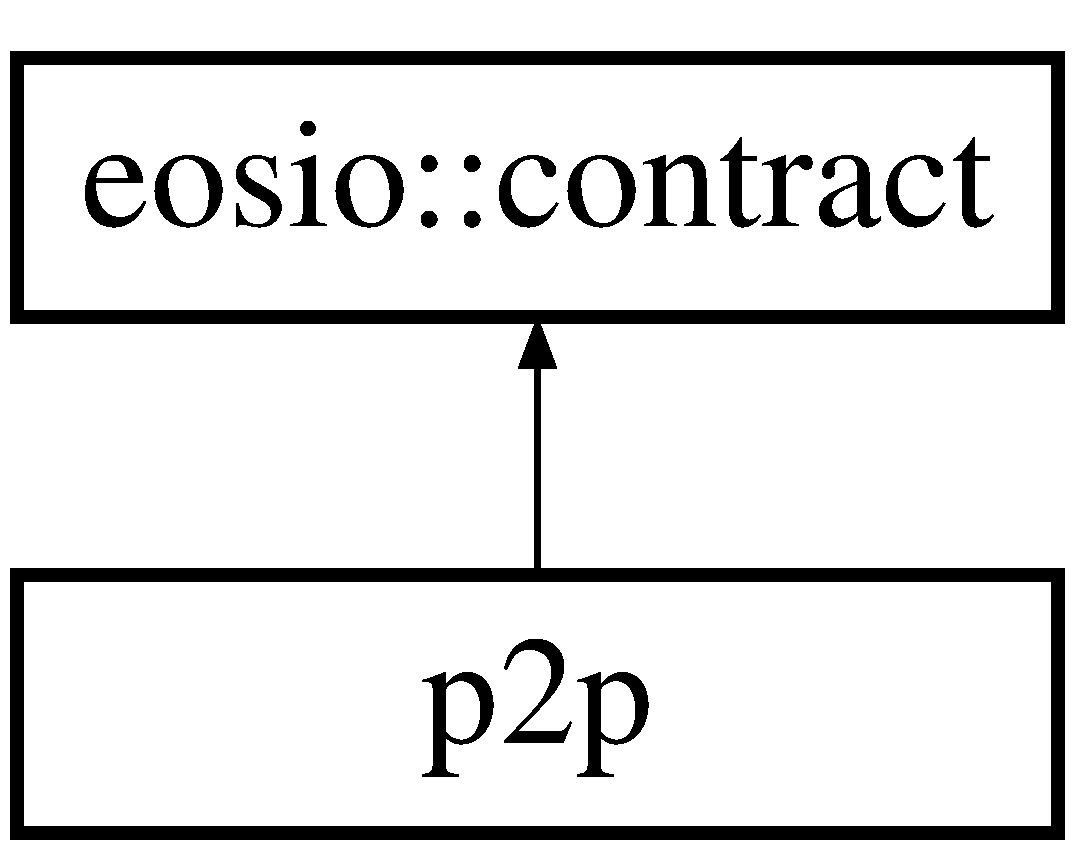
\includegraphics[height=2.000000cm]{de/d47/classp2p}
\end{center}
\end{figure}
\doxysubsection*{Data Structures}
\begin{DoxyCompactItemize}
\item 
struct \mbox{\hyperlink{structp2p_1_1balance}{balance}}
\begin{DoxyCompactList}\small\item\em Таблица промежуточного хранения балансов пользователей. \end{DoxyCompactList}\item 
struct \mbox{\hyperlink{structp2p_1_1bbonuses}{bbonuses}}
\begin{DoxyCompactList}\small\item\em Таблица резервов контракта для выплат бонусов в реферальную сеть \end{DoxyCompactList}\item 
struct \mbox{\hyperlink{structp2p_1_1counts}{counts}}
\begin{DoxyCompactList}\small\item\em Таблица счётчиков ордеров \end{DoxyCompactList}\item 
struct \mbox{\hyperlink{structp2p_1_1guests}{guests}}
\begin{DoxyCompactList}\small\item\em Таблица доступа к записям гостей платформы \end{DoxyCompactList}\item 
struct \mbox{\hyperlink{structp2p_1_1orders}{orders}}
\begin{DoxyCompactList}\small\item\em Таблица ордеров \end{DoxyCompactList}\item 
struct \mbox{\hyperlink{structp2p_1_1usdrates}{usdrates}}
\begin{DoxyCompactList}\small\item\em Таблица содержит курсы конвертации к доллару. \end{DoxyCompactList}\item 
struct \mbox{\hyperlink{structp2p_1_1usdrates2}{usdrates2}}
\begin{DoxyCompactList}\small\item\em Таблица расширения usdrates с указанием даты установки первого курса \end{DoxyCompactList}\item 
struct \mbox{\hyperlink{structp2p_1_1vesting}{vesting}}
\begin{DoxyCompactList}\small\item\em Таблица вестинг-\/балансов пользователей \end{DoxyCompactList}\end{DoxyCompactItemize}
\doxysubsection*{Public Types}
\begin{DoxyCompactItemize}
\item 
\mbox{\Hypertarget{classp2p_a562223292a6b99a97d486136b2eb0d9e}\label{classp2p_a562223292a6b99a97d486136b2eb0d9e}} 
typedef eosio\+::multi\+\_\+index$<$\char`\"{}balance\char`\"{}\+\_\+n, \mbox{\hyperlink{structp2p_1_1balance}{balance}}, eosio\+::indexed\+\_\+by$<$ \char`\"{}byconsym\char`\"{}\+\_\+n, eosio\+::const\+\_\+mem\+\_\+fun$<$ \mbox{\hyperlink{structp2p_1_1balance}{balance}}, uint128\+\_\+t, \&balance\+::byconsym $>$ $>$ $>$ {\bfseries balances\+\_\+index}
\item 
\mbox{\Hypertarget{classp2p_a6bef060ed784c193c2a60b397c869c29}\label{classp2p_a6bef060ed784c193c2a60b397c869c29}} 
typedef eosio\+::multi\+\_\+index$<$\char`\"{}counts\char`\"{}\+\_\+n, \mbox{\hyperlink{structp2p_1_1counts}{counts}} $>$ {\bfseries counts\+\_\+index}
\item 
\mbox{\Hypertarget{classp2p_af7e337013ebdcc44b420a6d55d0d385f}\label{classp2p_af7e337013ebdcc44b420a6d55d0d385f}} 
typedef eosio\+::multi\+\_\+index$<$ \char`\"{}orders\char`\"{}\+\_\+n, \mbox{\hyperlink{structp2p_1_1orders}{orders}}, eosio\+::indexed\+\_\+by$<$\char`\"{}bycurrcode\char`\"{}\+\_\+n, eosio\+::const\+\_\+mem\+\_\+fun$<$ \mbox{\hyperlink{structp2p_1_1orders}{orders}}, uint64\+\_\+t, \&\mbox{\hyperlink{structp2p_1_1orders_ab6f05a725122c94d3f2dcfaf24322c47}{orders\+::bycurrcode}} $>$ $>$, eosio\+::indexed\+\_\+by$<$\char`\"{}byparentid\char`\"{}\+\_\+n, eosio\+::const\+\_\+mem\+\_\+fun$<$ \mbox{\hyperlink{structp2p_1_1orders}{orders}}, uint64\+\_\+t, \&\mbox{\hyperlink{structp2p_1_1orders_a2b790da517561e8a593b6c56d63c4cfd}{orders\+::byparentid}} $>$ $>$, eosio\+::indexed\+\_\+by$<$\char`\"{}bytype\char`\"{}\+\_\+n, eosio\+::const\+\_\+mem\+\_\+fun$<$ \mbox{\hyperlink{structp2p_1_1orders}{orders}}, uint64\+\_\+t, \&\mbox{\hyperlink{structp2p_1_1orders_a17505cc3759a5ba5099f490c982535e1}{orders\+::bytype}} $>$ $>$, eosio\+::indexed\+\_\+by$<$\char`\"{}bycreator\char`\"{}\+\_\+n, eosio\+::const\+\_\+mem\+\_\+fun$<$ \mbox{\hyperlink{structp2p_1_1orders}{orders}}, uint64\+\_\+t, \&\mbox{\hyperlink{structp2p_1_1orders_a91b49c417f79ef405982bfe348651a98}{orders\+::bycreator}} $>$ $>$, eosio\+::indexed\+\_\+by$<$\char`\"{}bycurator\char`\"{}\+\_\+n, eosio\+::const\+\_\+mem\+\_\+fun$<$ \mbox{\hyperlink{structp2p_1_1orders}{orders}}, uint64\+\_\+t, \&\mbox{\hyperlink{structp2p_1_1orders_a76fa8b54f391ccd2e29b640d4c0199df}{orders\+::bycurator}} $>$ $>$, eosio\+::indexed\+\_\+by$<$\char`\"{}bystatus\char`\"{}\+\_\+n, eosio\+::const\+\_\+mem\+\_\+fun$<$ \mbox{\hyperlink{structp2p_1_1orders}{orders}}, uint64\+\_\+t, \&\mbox{\hyperlink{structp2p_1_1orders_a31e70a285fb324d4ee07b1b149debff3}{orders\+::bystatus}} $>$ $>$, eosio\+::indexed\+\_\+by$<$\char`\"{}byexpr\char`\"{}\+\_\+n, eosio\+::const\+\_\+mem\+\_\+fun$<$ \mbox{\hyperlink{structp2p_1_1orders}{orders}}, uint64\+\_\+t, \&\mbox{\hyperlink{structp2p_1_1orders_a8cf94dfb0902511c6baae1dd0434dcbf}{orders\+::byexpr}} $>$ $>$, eosio\+::indexed\+\_\+by$<$\char`\"{}bycreated\char`\"{}\+\_\+n, eosio\+::const\+\_\+mem\+\_\+fun$<$ \mbox{\hyperlink{structp2p_1_1orders}{orders}}, uint64\+\_\+t, \&\mbox{\hyperlink{structp2p_1_1orders_a6eab9cb4d0f7b605aef8856aad730fe5}{orders\+::bycreated}} $>$ $>$ $>$ {\bfseries orders\+\_\+index}
\item 
\mbox{\Hypertarget{classp2p_ac0dc7fa780d52c554aea91ab34bb3cfb}\label{classp2p_ac0dc7fa780d52c554aea91ab34bb3cfb}} 
typedef eosio\+::multi\+\_\+index$<$\char`\"{}usdrates\char`\"{}\+\_\+n, \mbox{\hyperlink{structp2p_1_1usdrates}{usdrates}}, eosio\+::indexed\+\_\+by$<$ \char`\"{}byconsym\char`\"{}\+\_\+n, eosio\+::const\+\_\+mem\+\_\+fun$<$ \mbox{\hyperlink{structp2p_1_1usdrates}{usdrates}}, uint128\+\_\+t, \&\mbox{\hyperlink{structp2p_1_1usdrates_a6d13bdd9e62d26ca68146e642e330099}{usdrates\+::byconsym}} $>$ $>$ $>$ {\bfseries usdrates\+\_\+index}
\item 
\mbox{\Hypertarget{classp2p_abbacbe5996794991fcbfb554dae6dc41}\label{classp2p_abbacbe5996794991fcbfb554dae6dc41}} 
typedef eosio\+::multi\+\_\+index$<$\char`\"{}usdrates2\char`\"{}\+\_\+n, \mbox{\hyperlink{structp2p_1_1usdrates2}{usdrates2}} $>$ {\bfseries usdrates2\+\_\+index}
\item 
\mbox{\Hypertarget{classp2p_ad2b234c3e4a379adfeebb42efe3fdb25}\label{classp2p_ad2b234c3e4a379adfeebb42efe3fdb25}} 
typedef eosio\+::multi\+\_\+index$<$\char`\"{}bbonuses\char`\"{}\+\_\+n, \mbox{\hyperlink{structp2p_1_1bbonuses}{bbonuses}} $>$ {\bfseries bbonuses\+\_\+index}
\item 
\mbox{\Hypertarget{classp2p_a9e10c97b92e817371f627c84094dce39}\label{classp2p_a9e10c97b92e817371f627c84094dce39}} 
typedef eosio\+::multi\+\_\+index$<$\char`\"{}vesting\char`\"{}\+\_\+n, \mbox{\hyperlink{structp2p_1_1vesting}{vesting}} $>$ {\bfseries vesting\+\_\+index}
\item 
\mbox{\Hypertarget{classp2p_a08507c2c104ad7e99765afd19d4fdd10}\label{classp2p_a08507c2c104ad7e99765afd19d4fdd10}} 
typedef eosio\+::multi\+\_\+index$<$\char`\"{}guests\char`\"{}\+\_\+n, \mbox{\hyperlink{structp2p_1_1guests}{guests}}, eosio\+::indexed\+\_\+by$<$ \char`\"{}byexpr\char`\"{}\+\_\+n, eosio\+::const\+\_\+mem\+\_\+fun$<$ \mbox{\hyperlink{structp2p_1_1guests}{guests}}, uint64\+\_\+t, \&guests\+::byexpr $>$ $>$, eosio\+::indexed\+\_\+by$<$ \char`\"{}byreg\char`\"{}\+\_\+n, eosio\+::const\+\_\+mem\+\_\+fun$<$ \mbox{\hyperlink{structp2p_1_1guests}{guests}}, uint64\+\_\+t, \&guests\+::byreg $>$ $>$ $>$ {\bfseries guests\+\_\+index}
\end{DoxyCompactItemize}
\doxysubsection*{Public Member Functions}
\begin{DoxyCompactItemize}
\item 
\mbox{\Hypertarget{classp2p_af05b8ff51661058078be1b96eb2bccb0}\label{classp2p_af05b8ff51661058078be1b96eb2bccb0}} 
{\bfseries p2p} (eosio\+::name receiver, eosio\+::name code, eosio\+::datastream$<$ const char $\ast$ $>$ ds)
\item 
\mbox{\Hypertarget{classp2p_a1ba9938186b683d21e39ae021d7a0a6f}\label{classp2p_a1ba9938186b683d21e39ae021d7a0a6f}} 
void {\bfseries apply} (uint64\+\_\+t receiver, uint64\+\_\+t code, uint64\+\_\+t action)
\item 
void \mbox{\hyperlink{group__public__actions_ga0b05f55568e9469d33379512b29a116a}{createorder}} (name username, uint64\+\_\+t parent\+\_\+id, name type, eosio\+::name root\+\_\+contract, eosio\+::asset root\+\_\+quantity, eosio\+::name quote\+\_\+type, double quote\+\_\+rate, eosio\+::name quote\+\_\+contract, eosio\+::asset quote\+\_\+quantity, eosio\+::name out\+\_\+type, double out\+\_\+rate, eosio\+::name out\+\_\+contract, eosio\+::asset out\+\_\+quantity, std\+::string details)
\begin{DoxyCompactList}\small\item\em Метод создания ордера \end{DoxyCompactList}\item 
void \mbox{\hyperlink{group__public__actions_gab7d91c105e22cc794a42cb12d996d0cb}{accept}} (name username, uint64\+\_\+t id, std\+::string details)
\begin{DoxyCompactList}\small\item\em Метод подтверждения факта присутствия и начало сделки \end{DoxyCompactList}\item 
void \mbox{\hyperlink{group__public__actions_ga4562d6493c57589bf2259f119481d39a}{approve}} (name username, uint64\+\_\+t id)
\begin{DoxyCompactList}\small\item\em Метод утверждения завершенного ордера \end{DoxyCompactList}\item 
void \mbox{\hyperlink{group__public__actions_gaa1abaf488133faec3fae6c6c9c9917c2}{confirm}} (name username, uint64\+\_\+t id)
\begin{DoxyCompactList}\small\item\em Метод подтверждения факта платежа \end{DoxyCompactList}\item 
void \mbox{\hyperlink{group__public__actions_gaf81f265e37d1f1572a9a5fa17fa99f32}{cancel}} (name username, uint64\+\_\+t id)
\begin{DoxyCompactList}\small\item\em Метод отмены ордера \end{DoxyCompactList}\item 
void \mbox{\hyperlink{group__public__actions_ga4f0c0c376096f7a73b21b39f0dc58d1d}{dispute}} (name username, uint64\+\_\+t id)
\begin{DoxyCompactList}\small\item\em Метод создания спора \end{DoxyCompactList}\item 
void \mbox{\hyperlink{group__public__actions_ga805effb2c6e15ab30e7f36bf13558910}{del}} (name username, uint64\+\_\+t id)
\begin{DoxyCompactList}\small\item\em Метод удаления завершенной сделки из оперативной памяти \end{DoxyCompactList}\item 
void \mbox{\hyperlink{group__public__actions_ga432842119735888f862933882e6a4da6}{setrate}} (eosio\+::name out\+\_\+contract, eosio\+::asset out\+\_\+asset, double rate)
\begin{DoxyCompactList}\small\item\em Метод установки курса обмена к USD. \end{DoxyCompactList}\item 
void \mbox{\hyperlink{group__public__actions_ga6684d814e1a17f87c492e2b394cc1846}{uprate}} (eosio\+::name out\+\_\+contract, eosio\+::asset out\+\_\+asset)
\begin{DoxyCompactList}\small\item\em Метод увеличения курса обмена системного токена \end{DoxyCompactList}\item 
void \mbox{\hyperlink{group__public__actions_gabea413390558d072de45f9ff47217ff8}{delrate}} (uint64\+\_\+t id)
\begin{DoxyCompactList}\small\item\em Метод удаление курса \end{DoxyCompactList}\item 
void \mbox{\hyperlink{group__public__actions_ga6ef3ff3b489159e054195c1d8fbd7092}{delvesting}} (eosio\+::name owner, uint64\+\_\+t id)
\begin{DoxyCompactList}\small\item\em Метод удаление вестинг-\/баланса \end{DoxyCompactList}\item 
void \mbox{\hyperlink{group__public__actions_ga4f3c89b4ae21f54b6e16334e681a7860}{setbrate}} (eosio\+::name host, double distribution\+\_\+rate)
\begin{DoxyCompactList}\small\item\em Метод установки бонусного курса \end{DoxyCompactList}\item 
void \mbox{\hyperlink{group__public__actions_ga2cb80d56fbb68ac3ccc688112d86532a}{refreshsh}} (eosio\+::name owner, uint64\+\_\+t id)
\begin{DoxyCompactList}\small\item\em Метод обновления вестинг-\/баланса. ~\newline
 \end{DoxyCompactList}\item 
void \mbox{\hyperlink{group__public__actions_gadb4fde78468ee3b060717a785febdcc4}{withdrawsh}} (eosio\+::name owner, uint64\+\_\+t id)
\begin{DoxyCompactList}\small\item\em Вывод вестинг-\/баланса \end{DoxyCompactList}\end{DoxyCompactItemize}
\doxysubsection*{Static Public Member Functions}
\begin{DoxyCompactItemize}
\item 
\mbox{\Hypertarget{classp2p_ac36f6042dcb8942679dddbf672684ddc}\label{classp2p_ac36f6042dcb8942679dddbf672684ddc}} 
static void {\bfseries add\+\_\+balance} (eosio\+::name payer, eosio\+::asset quantity, eosio\+::name contract)
\item 
\mbox{\Hypertarget{classp2p_afc44fa7dedaeea9559af5f70445b5218}\label{classp2p_afc44fa7dedaeea9559af5f70445b5218}} 
static void {\bfseries sub\+\_\+balance} (eosio\+::name username, eosio\+::asset quantity, eosio\+::name contract)
\item 
\mbox{\Hypertarget{classp2p_aa6f449f9ebec47b6741ed3497a3b92f9}\label{classp2p_aa6f449f9ebec47b6741ed3497a3b92f9}} 
static void {\bfseries addbbal} (eosio\+::name host, eosio\+::name contract, eosio\+::asset quantity)
\item 
\mbox{\Hypertarget{classp2p_a9bbb48f7000e2ad2c901fe04f3e7f024}\label{classp2p_a9bbb48f7000e2ad2c901fe04f3e7f024}} 
static void {\bfseries subbbal} (eosio\+::name host, eosio\+::name contract, eosio\+::asset quantity)
\item 
\mbox{\Hypertarget{classp2p_a0b427c0584a5dd22a924273d3476dfd7}\label{classp2p_a0b427c0584a5dd22a924273d3476dfd7}} 
static void {\bfseries make\+\_\+vesting\+\_\+action} (eosio\+::name owner, eosio\+::name contract, eosio\+::asset amount)
\item 
\mbox{\Hypertarget{classp2p_ac62758f88566e5dafc0804182f324658}\label{classp2p_ac62758f88566e5dafc0804182f324658}} 
static void {\bfseries check\+\_\+bonuse\+\_\+system} (eosio\+::name creator, eosio\+::name reciever, eosio\+::asset quantity)
\item 
\mbox{\Hypertarget{classp2p_a5a20e06fb911402d5e343389bdf944d4}\label{classp2p_a5a20e06fb911402d5e343389bdf944d4}} 
static void {\bfseries check\+\_\+guest\+\_\+and\+\_\+gift\+\_\+account} (eosio\+::name username, eosio\+::name contract, eosio\+::asset amount)
\item 
\mbox{\Hypertarget{classp2p_a6277838ad086e92577864a4c59ec3e6c}\label{classp2p_a6277838ad086e92577864a4c59ec3e6c}} 
static uint64\+\_\+t {\bfseries get\+\_\+order\+\_\+id} ()
\item 
\mbox{\Hypertarget{classp2p_a4aa15958215b4647e9adc4ed3d53af8c}\label{classp2p_a4aa15958215b4647e9adc4ed3d53af8c}} 
static uint128\+\_\+t {\bfseries combine\+\_\+ids} (const uint64\+\_\+t \&x, const uint64\+\_\+t \&y)
\end{DoxyCompactItemize}
\doxysubsection*{Static Public Attributes}
\begin{DoxyCompactItemize}
\item 
static constexpr eosio\+::name \mbox{\hyperlink{group__public__consts_gade9426b6e05cdb60d41e808717199b89}{\+\_\+me}} = \char`\"{}p2p\char`\"{}\+\_\+n
\item 
static constexpr eosio\+::name \mbox{\hyperlink{classp2p_aa5528a78186585c3a033d89b6c027a5b}{\+\_\+curator}} = \char`\"{}p2p\char`\"{}\+\_\+n
\item 
static constexpr eosio\+::name \mbox{\hyperlink{classp2p_abaf26be47ba132e33bdadf4a6f65a052}{\+\_\+rater}} = \char`\"{}rater\char`\"{}\+\_\+n
\item 
static constexpr eosio\+::symbol \mbox{\hyperlink{classp2p_afe8d32633b8a87ce35209184d222f6de}{\+\_\+\+SYM}} = eosio\+::symbol(eosio\+::symbol\+\_\+code(\char`\"{}FLOWER\char`\"{}), 4)
\item 
static constexpr eosio\+::name \mbox{\hyperlink{classp2p_a582434add36ca36a326bdab9e7c8cb4e}{\+\_\+core}} = \char`\"{}unicore\char`\"{}\+\_\+n
\item 
static const uint64\+\_\+t \mbox{\hyperlink{classp2p_a6a7a6607c93e930cfa3984a8c318942b}{\+\_\+\+PERCENTS\+\_\+\+PER\+\_\+\+MONTH}} = 42
\item 
static const bool \mbox{\hyperlink{classp2p_a738ddf63d1276c74f28b7d2f51ba1475}{\+\_\+\+ENABLE\+\_\+\+GROWHT}} = false
\item 
static const bool \mbox{\hyperlink{classp2p_a817118e4e422393acc35439edb0187af}{\+\_\+\+ENABLE\+\_\+\+VESTING}} = false
\item 
static const uint64\+\_\+t \mbox{\hyperlink{classp2p_af52bcfc4c42cb8a001ab4935d06539c0}{\+\_\+\+VESTING\+\_\+\+SECONDS}} = 15770000
\item 
static constexpr eosio\+::name \mbox{\hyperlink{classp2p_aaf70e52c0f57cc4fa3d9d7fd0e8f0d99}{\+\_\+\+CORE\+\_\+\+SALE\+\_\+\+ACCOUNT}} = \char`\"{}core\char`\"{}\+\_\+n
\item 
static constexpr eosio\+::name \mbox{\hyperlink{classp2p_ad3c9fd465ea37d16657bd9910c631d22}{\+\_\+\+REGISTRATOR\+\_\+\+ACCOUNT}} = \char`\"{}registrator\char`\"{}\+\_\+n
\item 
static const uint64\+\_\+t \mbox{\hyperlink{classp2p_ada18e95b855fa10dc57a33620b4dd51d}{\+\_\+\+GIFT\+\_\+\+ACCOUNT\+\_\+\+FROM\+\_\+\+AMOUNT}} = 100000
\item 
static const uint64\+\_\+t \mbox{\hyperlink{classp2p_a714001f0f556d0db16b3746fa2261ddb}{\+\_\+\+ORDER\+\_\+\+EXPIRATION}} = 30 $\ast$ 60
\item 
static constexpr double \mbox{\hyperlink{classp2p_a41fd0523f7a4103ea012c69c376d0823}{\+\_\+\+START\+\_\+\+RATE}} = 0.\+2
\end{DoxyCompactItemize}


\doxysubsection{Detailed Description}
Начните ознакомление здесь. 

\doxysubsection{Field Documentation}
\mbox{\Hypertarget{classp2p_a582434add36ca36a326bdab9e7c8cb4e}\label{classp2p_a582434add36ca36a326bdab9e7c8cb4e}} 
\index{p2p@{p2p}!\_core@{\_core}}
\index{\_core@{\_core}!p2p@{p2p}}
\doxysubsubsection{\texorpdfstring{\_core}{\_core}}
{\footnotesize\ttfamily constexpr eosio\+::name p2p\+::\+\_\+core = \char`\"{}unicore\char`\"{}\+\_\+n\hspace{0.3cm}{\ttfamily [static]}, {\ttfamily [constexpr]}}

имя аккаунта распределения реферальных бонусов в сеть \mbox{\Hypertarget{classp2p_aaf70e52c0f57cc4fa3d9d7fd0e8f0d99}\label{classp2p_aaf70e52c0f57cc4fa3d9d7fd0e8f0d99}} 
\index{p2p@{p2p}!\_CORE\_SALE\_ACCOUNT@{\_CORE\_SALE\_ACCOUNT}}
\index{\_CORE\_SALE\_ACCOUNT@{\_CORE\_SALE\_ACCOUNT}!p2p@{p2p}}
\doxysubsubsection{\texorpdfstring{\_CORE\_SALE\_ACCOUNT}{\_CORE\_SALE\_ACCOUNT}}
{\footnotesize\ttfamily constexpr eosio\+::name p2p\+::\+\_\+\+CORE\+\_\+\+SALE\+\_\+\+ACCOUNT = \char`\"{}core\char`\"{}\+\_\+n\hspace{0.3cm}{\ttfamily [static]}, {\ttfamily [constexpr]}}

аккаунт системного продавца токенов, в сделке к которым срабатывает вестинг \mbox{\Hypertarget{classp2p_aa5528a78186585c3a033d89b6c027a5b}\label{classp2p_aa5528a78186585c3a033d89b6c027a5b}} 
\index{p2p@{p2p}!\_curator@{\_curator}}
\index{\_curator@{\_curator}!p2p@{p2p}}
\doxysubsubsection{\texorpdfstring{\_curator}{\_curator}}
{\footnotesize\ttfamily constexpr eosio\+::name p2p\+::\+\_\+curator = \char`\"{}p2p\char`\"{}\+\_\+n\hspace{0.3cm}{\ttfamily [static]}, {\ttfamily [constexpr]}}

дефолтное имя аккаунта куратора всех сделок \mbox{\Hypertarget{classp2p_a738ddf63d1276c74f28b7d2f51ba1475}\label{classp2p_a738ddf63d1276c74f28b7d2f51ba1475}} 
\index{p2p@{p2p}!\_ENABLE\_GROWHT@{\_ENABLE\_GROWHT}}
\index{\_ENABLE\_GROWHT@{\_ENABLE\_GROWHT}!p2p@{p2p}}
\doxysubsubsection{\texorpdfstring{\_ENABLE\_GROWHT}{\_ENABLE\_GROWHT}}
{\footnotesize\ttfamily const bool p2p\+::\+\_\+\+ENABLE\+\_\+\+GROWHT = false\hspace{0.3cm}{\ttfamily [static]}}

флаг подключения автоматического роста курса, допускающего вызов метода uprate от системного контракта eosio \mbox{\Hypertarget{classp2p_a817118e4e422393acc35439edb0187af}\label{classp2p_a817118e4e422393acc35439edb0187af}} 
\index{p2p@{p2p}!\_ENABLE\_VESTING@{\_ENABLE\_VESTING}}
\index{\_ENABLE\_VESTING@{\_ENABLE\_VESTING}!p2p@{p2p}}
\doxysubsubsection{\texorpdfstring{\_ENABLE\_VESTING}{\_ENABLE\_VESTING}}
{\footnotesize\ttfamily const bool p2p\+::\+\_\+\+ENABLE\+\_\+\+VESTING = false\hspace{0.3cm}{\ttfamily [static]}}

флаг подключения режима вестинга для совершенных покупок у аккаунта \+\_\+\+CORE\+\_\+\+SALE\+\_\+\+ACCOUNT \mbox{\Hypertarget{classp2p_ada18e95b855fa10dc57a33620b4dd51d}\label{classp2p_ada18e95b855fa10dc57a33620b4dd51d}} 
\index{p2p@{p2p}!\_GIFT\_ACCOUNT\_FROM\_AMOUNT@{\_GIFT\_ACCOUNT\_FROM\_AMOUNT}}
\index{\_GIFT\_ACCOUNT\_FROM\_AMOUNT@{\_GIFT\_ACCOUNT\_FROM\_AMOUNT}!p2p@{p2p}}
\doxysubsubsection{\texorpdfstring{\_GIFT\_ACCOUNT\_FROM\_AMOUNT}{\_GIFT\_ACCOUNT\_FROM\_AMOUNT}}
{\footnotesize\ttfamily const uint64\+\_\+t p2p\+::\+\_\+\+GIFT\+\_\+\+ACCOUNT\+\_\+\+FROM\+\_\+\+AMOUNT = 100000\hspace{0.3cm}{\ttfamily [static]}}

подарок в виде аккаунта партнера осуществляется, если гость совершает покупку на сумму более, чем указано здесь (с учётом точности) \mbox{\Hypertarget{classp2p_a714001f0f556d0db16b3746fa2261ddb}\label{classp2p_a714001f0f556d0db16b3746fa2261ddb}} 
\index{p2p@{p2p}!\_ORDER\_EXPIRATION@{\_ORDER\_EXPIRATION}}
\index{\_ORDER\_EXPIRATION@{\_ORDER\_EXPIRATION}!p2p@{p2p}}
\doxysubsubsection{\texorpdfstring{\_ORDER\_EXPIRATION}{\_ORDER\_EXPIRATION}}
{\footnotesize\ttfamily const uint64\+\_\+t p2p\+::\+\_\+\+ORDER\+\_\+\+EXPIRATION = 30 $\ast$ 60\hspace{0.3cm}{\ttfamily [static]}}

время до истечения срока давности ордера \mbox{\Hypertarget{classp2p_a6a7a6607c93e930cfa3984a8c318942b}\label{classp2p_a6a7a6607c93e930cfa3984a8c318942b}} 
\index{p2p@{p2p}!\_PERCENTS\_PER\_MONTH@{\_PERCENTS\_PER\_MONTH}}
\index{\_PERCENTS\_PER\_MONTH@{\_PERCENTS\_PER\_MONTH}!p2p@{p2p}}
\doxysubsubsection{\texorpdfstring{\_PERCENTS\_PER\_MONTH}{\_PERCENTS\_PER\_MONTH}}
{\footnotesize\ttfamily const uint64\+\_\+t p2p\+::\+\_\+\+PERCENTS\+\_\+\+PER\+\_\+\+MONTH = 42\hspace{0.3cm}{\ttfamily [static]}}

если рост курса системного токена подключен, то растёт с указанной здесь скоростью \mbox{\Hypertarget{classp2p_abaf26be47ba132e33bdadf4a6f65a052}\label{classp2p_abaf26be47ba132e33bdadf4a6f65a052}} 
\index{p2p@{p2p}!\_rater@{\_rater}}
\index{\_rater@{\_rater}!p2p@{p2p}}
\doxysubsubsection{\texorpdfstring{\_rater}{\_rater}}
{\footnotesize\ttfamily constexpr eosio\+::name p2p\+::\+\_\+rater = \char`\"{}rater\char`\"{}\+\_\+n\hspace{0.3cm}{\ttfamily [static]}, {\ttfamily [constexpr]}}

имя аккаунта поставщика курсов \mbox{\Hypertarget{classp2p_ad3c9fd465ea37d16657bd9910c631d22}\label{classp2p_ad3c9fd465ea37d16657bd9910c631d22}} 
\index{p2p@{p2p}!\_REGISTRATOR\_ACCOUNT@{\_REGISTRATOR\_ACCOUNT}}
\index{\_REGISTRATOR\_ACCOUNT@{\_REGISTRATOR\_ACCOUNT}!p2p@{p2p}}
\doxysubsubsection{\texorpdfstring{\_REGISTRATOR\_ACCOUNT}{\_REGISTRATOR\_ACCOUNT}}
{\footnotesize\ttfamily constexpr eosio\+::name p2p\+::\+\_\+\+REGISTRATOR\+\_\+\+ACCOUNT = \char`\"{}registrator\char`\"{}\+\_\+n\hspace{0.3cm}{\ttfamily [static]}, {\ttfamily [constexpr]}}

аккаунт контракта регистратора, хранящего таблицу с гостями для подарочного выкупа \mbox{\Hypertarget{classp2p_a41fd0523f7a4103ea012c69c376d0823}\label{classp2p_a41fd0523f7a4103ea012c69c376d0823}} 
\index{p2p@{p2p}!\_START\_RATE@{\_START\_RATE}}
\index{\_START\_RATE@{\_START\_RATE}!p2p@{p2p}}
\doxysubsubsection{\texorpdfstring{\_START\_RATE}{\_START\_RATE}}
{\footnotesize\ttfamily constexpr double p2p\+::\+\_\+\+START\+\_\+\+RATE = 0.\+2\hspace{0.3cm}{\ttfamily [static]}, {\ttfamily [constexpr]}}

начальный курс старта роста системного токена относительно USD \mbox{\Hypertarget{classp2p_afe8d32633b8a87ce35209184d222f6de}\label{classp2p_afe8d32633b8a87ce35209184d222f6de}} 
\index{p2p@{p2p}!\_SYM@{\_SYM}}
\index{\_SYM@{\_SYM}!p2p@{p2p}}
\doxysubsubsection{\texorpdfstring{\_SYM}{\_SYM}}
{\footnotesize\ttfamily constexpr eosio\+::symbol p2p\+::\+\_\+\+SYM = eosio\+::symbol(eosio\+::symbol\+\_\+code(\char`\"{}FLOWER\char`\"{}), 4)\hspace{0.3cm}{\ttfamily [static]}, {\ttfamily [constexpr]}}

системный токен \mbox{\Hypertarget{classp2p_af52bcfc4c42cb8a001ab4935d06539c0}\label{classp2p_af52bcfc4c42cb8a001ab4935d06539c0}} 
\index{p2p@{p2p}!\_VESTING\_SECONDS@{\_VESTING\_SECONDS}}
\index{\_VESTING\_SECONDS@{\_VESTING\_SECONDS}!p2p@{p2p}}
\doxysubsubsection{\texorpdfstring{\_VESTING\_SECONDS}{\_VESTING\_SECONDS}}
{\footnotesize\ttfamily const uint64\+\_\+t p2p\+::\+\_\+\+VESTING\+\_\+\+SECONDS = 15770000\hspace{0.3cm}{\ttfamily [static]}}

продолжительность вестинга в секундах 

The documentation for this class was generated from the following files\+:\begin{DoxyCompactItemize}
\item 
p2p.\+hpp\item 
p2p.\+cpp\end{DoxyCompactItemize}

\hypertarget{structp2p_1_1usdrates}{}\doxysection{p2p\+::usdrates Struct Reference}
\label{structp2p_1_1usdrates}\index{p2p::usdrates@{p2p::usdrates}}


Таблица содержит курсы конвертации к доллару.  




{\ttfamily \#include $<$p2p.\+hpp$>$}

\doxysubsection*{Public Member Functions}
\begin{DoxyCompactItemize}
\item 
uint64\+\_\+t \mbox{\hyperlink{structp2p_1_1usdrates_a8bdf953b105c26b52b6fe3be2b910925}{primary\+\_\+key}} () const
\item 
uint128\+\_\+t \mbox{\hyperlink{structp2p_1_1usdrates_a6d13bdd9e62d26ca68146e642e330099}{byconsym}} () const
\end{DoxyCompactItemize}
\doxysubsection*{Data Fields}
\begin{DoxyCompactItemize}
\item 
uint64\+\_\+t \mbox{\hyperlink{structp2p_1_1usdrates_a5f755d95b0efa7942636fddfae33db2f}{id}}
\item 
eosio\+::name \mbox{\hyperlink{structp2p_1_1usdrates_a6e1aa8746a552939956d3aa3e93782d9}{out\+\_\+contract}}
\item 
eosio\+::asset \mbox{\hyperlink{structp2p_1_1usdrates_ac6ba77785a025d183b2378d5b1bb7f69}{out\+\_\+asset}}
\item 
double \mbox{\hyperlink{structp2p_1_1usdrates_a4a0439519abb54675759686a1b5fe43a}{rate}}
\item 
eosio\+::time\+\_\+point\+\_\+sec \mbox{\hyperlink{structp2p_1_1usdrates_a79bb6e9971e40371c8003013887bf294}{updated\+\_\+at}}
\end{DoxyCompactItemize}


\doxysubsection{Detailed Description}
Таблица содержит курсы конвертации к доллару. 

CONTRACT = \+\_\+me, SCOPE = \+\_\+me, TABLE = usdrates

Курсы обновляются аккаунтом rater методом setrate или системным контрактом eosio методом uprate. 

\doxysubsection{Member Function Documentation}
\mbox{\Hypertarget{structp2p_1_1usdrates_a6d13bdd9e62d26ca68146e642e330099}\label{structp2p_1_1usdrates_a6d13bdd9e62d26ca68146e642e330099}} 
\index{p2p::usdrates@{p2p::usdrates}!byconsym@{byconsym}}
\index{byconsym@{byconsym}!p2p::usdrates@{p2p::usdrates}}
\doxysubsubsection{\texorpdfstring{byconsym()}{byconsym()}}
{\footnotesize\ttfamily uint128\+\_\+t p2p\+::usdrates\+::byconsym (\begin{DoxyParamCaption}{ }\end{DoxyParamCaption}) const\hspace{0.3cm}{\ttfamily [inline]}}

(out\+\_\+contract, out\+\_\+asset.\+symbol) -\/ комбинированный secondary\+\_\+key для получения курса по имени выходного контракта и символу \mbox{\Hypertarget{structp2p_1_1usdrates_a8bdf953b105c26b52b6fe3be2b910925}\label{structp2p_1_1usdrates_a8bdf953b105c26b52b6fe3be2b910925}} 
\index{p2p::usdrates@{p2p::usdrates}!primary\_key@{primary\_key}}
\index{primary\_key@{primary\_key}!p2p::usdrates@{p2p::usdrates}}
\doxysubsubsection{\texorpdfstring{primary\_key()}{primary\_key()}}
{\footnotesize\ttfamily uint64\+\_\+t p2p\+::usdrates\+::primary\+\_\+key (\begin{DoxyParamCaption}{ }\end{DoxyParamCaption}) const\hspace{0.3cm}{\ttfamily [inline]}}

id -\/ primary\+\_\+key 

\doxysubsection{Field Documentation}
\mbox{\Hypertarget{structp2p_1_1usdrates_a5f755d95b0efa7942636fddfae33db2f}\label{structp2p_1_1usdrates_a5f755d95b0efa7942636fddfae33db2f}} 
\index{p2p::usdrates@{p2p::usdrates}!id@{id}}
\index{id@{id}!p2p::usdrates@{p2p::usdrates}}
\doxysubsubsection{\texorpdfstring{id}{id}}
{\footnotesize\ttfamily uint64\+\_\+t p2p\+::usdrates\+::id}

идентификатор курса \mbox{\Hypertarget{structp2p_1_1usdrates_ac6ba77785a025d183b2378d5b1bb7f69}\label{structp2p_1_1usdrates_ac6ba77785a025d183b2378d5b1bb7f69}} 
\index{p2p::usdrates@{p2p::usdrates}!out\_asset@{out\_asset}}
\index{out\_asset@{out\_asset}!p2p::usdrates@{p2p::usdrates}}
\doxysubsubsection{\texorpdfstring{out\_asset}{out\_asset}}
{\footnotesize\ttfamily eosio\+::asset p2p\+::usdrates\+::out\+\_\+asset}

токен выхода \mbox{\Hypertarget{structp2p_1_1usdrates_a6e1aa8746a552939956d3aa3e93782d9}\label{structp2p_1_1usdrates_a6e1aa8746a552939956d3aa3e93782d9}} 
\index{p2p::usdrates@{p2p::usdrates}!out\_contract@{out\_contract}}
\index{out\_contract@{out\_contract}!p2p::usdrates@{p2p::usdrates}}
\doxysubsubsection{\texorpdfstring{out\_contract}{out\_contract}}
{\footnotesize\ttfamily eosio\+::name p2p\+::usdrates\+::out\+\_\+contract}

контракт выхода; если в конвертации используется внешняя валюта (например, фиатный RUB), контракт не устанавливается. Во внутренних конвертациях используется только при указании курса жетона ядра системы к доллару. \mbox{\Hypertarget{structp2p_1_1usdrates_a4a0439519abb54675759686a1b5fe43a}\label{structp2p_1_1usdrates_a4a0439519abb54675759686a1b5fe43a}} 
\index{p2p::usdrates@{p2p::usdrates}!rate@{rate}}
\index{rate@{rate}!p2p::usdrates@{p2p::usdrates}}
\doxysubsubsection{\texorpdfstring{rate}{rate}}
{\footnotesize\ttfamily double p2p\+::usdrates\+::rate}

курс токена выхода к доллару \mbox{\Hypertarget{structp2p_1_1usdrates_a79bb6e9971e40371c8003013887bf294}\label{structp2p_1_1usdrates_a79bb6e9971e40371c8003013887bf294}} 
\index{p2p::usdrates@{p2p::usdrates}!updated\_at@{updated\_at}}
\index{updated\_at@{updated\_at}!p2p::usdrates@{p2p::usdrates}}
\doxysubsubsection{\texorpdfstring{updated\_at}{updated\_at}}
{\footnotesize\ttfamily eosio\+::time\+\_\+point\+\_\+sec p2p\+::usdrates\+::updated\+\_\+at}

дата последнего обновления курса 

The documentation for this struct was generated from the following file\+:\begin{DoxyCompactItemize}
\item 
p2p.\+hpp\end{DoxyCompactItemize}

\hypertarget{structp2p_1_1usdrates2}{}\section{p2p\+:\+:usdrates2 Struct Reference}
\label{structp2p_1_1usdrates2}\index{p2p\+::usdrates2@{p2p\+::usdrates2}}


Таблица расширения usdrates с указанием даты установки первого курса  




{\ttfamily \#include $<$p2p.\+hpp$>$}

\subsection*{Public Member Functions}
\begin{DoxyCompactItemize}
\item 
uint64\+\_\+t \mbox{\hyperlink{structp2p_1_1usdrates2_aa3556a870e531f2a33d3a40ba45bc2da}{primary\+\_\+key}} () const
\end{DoxyCompactItemize}
\subsection*{Public Attributes}
\begin{DoxyCompactItemize}
\item 
uint64\+\_\+t \mbox{\hyperlink{structp2p_1_1usdrates2_aba230f3a86e3c9eb693c41d501378c22}{id}}
\item 
eosio\+::time\+\_\+point\+\_\+sec \mbox{\hyperlink{structp2p_1_1usdrates2_a2f8aa31571d84a178259fa42461cf140}{created\+\_\+at}}
\end{DoxyCompactItemize}


\subsection{Detailed Description}
Таблица расширения usdrates с указанием даты установки первого курса 

C\+O\+N\+T\+R\+A\+CT = \+\_\+me, S\+C\+O\+PE = \+\_\+me, T\+A\+B\+LE = \mbox{\hyperlink{structp2p_1_1usdrates2}{usdrates2}} 

\subsection{Member Function Documentation}
\mbox{\Hypertarget{structp2p_1_1usdrates2_aa3556a870e531f2a33d3a40ba45bc2da}\label{structp2p_1_1usdrates2_aa3556a870e531f2a33d3a40ba45bc2da}} 
\index{p2p\+::usdrates2@{p2p\+::usdrates2}!primary\+\_\+key@{primary\+\_\+key}}
\index{primary\+\_\+key@{primary\+\_\+key}!p2p\+::usdrates2@{p2p\+::usdrates2}}
\subsubsection{\texorpdfstring{primary\+\_\+key()}{primary\_key()}}
{\footnotesize\ttfamily uint64\+\_\+t p2p\+::usdrates2\+::primary\+\_\+key (\begin{DoxyParamCaption}{ }\end{DoxyParamCaption}) const\hspace{0.3cm}{\ttfamily [inline]}}

id -\/ primary\+\_\+key 

\subsection{Member Data Documentation}
\mbox{\Hypertarget{structp2p_1_1usdrates2_a2f8aa31571d84a178259fa42461cf140}\label{structp2p_1_1usdrates2_a2f8aa31571d84a178259fa42461cf140}} 
\index{p2p\+::usdrates2@{p2p\+::usdrates2}!created\+\_\+at@{created\+\_\+at}}
\index{created\+\_\+at@{created\+\_\+at}!p2p\+::usdrates2@{p2p\+::usdrates2}}
\subsubsection{\texorpdfstring{created\+\_\+at}{created\_at}}
{\footnotesize\ttfamily eosio\+::time\+\_\+point\+\_\+sec p2p\+::usdrates2\+::created\+\_\+at}

дата установки первого курса \mbox{\Hypertarget{structp2p_1_1usdrates2_aba230f3a86e3c9eb693c41d501378c22}\label{structp2p_1_1usdrates2_aba230f3a86e3c9eb693c41d501378c22}} 
\index{p2p\+::usdrates2@{p2p\+::usdrates2}!id@{id}}
\index{id@{id}!p2p\+::usdrates2@{p2p\+::usdrates2}}
\subsubsection{\texorpdfstring{id}{id}}
{\footnotesize\ttfamily uint64\+\_\+t p2p\+::usdrates2\+::id}

идентификатор курса 

The documentation for this struct was generated from the following file\+:\begin{DoxyCompactItemize}
\item 
p2p.\+hpp\end{DoxyCompactItemize}

\hypertarget{structp2p_1_1vesting}{}\doxysection{p2p\+::vesting Struct Reference}
\label{structp2p_1_1vesting}\index{p2p::vesting@{p2p::vesting}}


Таблица вестинг-\/балансов пользователей  




{\ttfamily \#include $<$p2p.\+hpp$>$}

\doxysubsection*{Public Member Functions}
\begin{DoxyCompactItemize}
\item 
uint64\+\_\+t \mbox{\hyperlink{structp2p_1_1vesting_a816764ab2ece434f3569aa4210d7442f}{primary\+\_\+key}} () const
\end{DoxyCompactItemize}
\doxysubsection*{Data Fields}
\begin{DoxyCompactItemize}
\item 
uint64\+\_\+t \mbox{\hyperlink{structp2p_1_1vesting_af92c78d429a89e9b6ce552ef480794d5}{id}}
\item 
eosio\+::name \mbox{\hyperlink{structp2p_1_1vesting_a46a58437b03f9c7947c76e91f358003e}{owner}}
\item 
eosio\+::name \mbox{\hyperlink{structp2p_1_1vesting_aa514aefb9ae797ecbf711997efb94d5b}{contract}}
\item 
eosio\+::time\+\_\+point\+\_\+sec \mbox{\hyperlink{structp2p_1_1vesting_ac2a702d706aa9146588fffb6113d1c79}{startat}}
\item 
uint64\+\_\+t \mbox{\hyperlink{structp2p_1_1vesting_a86ada5ec19fb224f483ab95bf5908547}{duration}}
\item 
eosio\+::asset \mbox{\hyperlink{structp2p_1_1vesting_a5a06c08d24cb3f9b929bc4285dd51179}{amount}}
\item 
eosio\+::asset \mbox{\hyperlink{structp2p_1_1vesting_a3759f66455f668a402c365554ad6550d}{available}}
\item 
eosio\+::asset \mbox{\hyperlink{structp2p_1_1vesting_a88ce3db1c7e1d53750a8d6e864da8c6c}{withdrawed}}
\end{DoxyCompactItemize}


\doxysubsection{Detailed Description}
Таблица вестинг-\/балансов пользователей 

CONTRACT = \+\_\+me, SCOPE = owner, TABLE = vesting

Пополняется контрактом в случае, если ключ \+\_\+\+ENABLE\+\_\+\+VESTING = TRUE на количество секунд в \+\_\+\+VESTING\+\_\+\+SECONDS, срабатывает только для аккаунта продавца \+\_\+\+CORE\+\_\+\+SALE\+\_\+\+ACCOUNT. Позволяет заморозить покупку токенов у компании на указанное количество секунд. 

\doxysubsection{Member Function Documentation}
\mbox{\Hypertarget{structp2p_1_1vesting_a816764ab2ece434f3569aa4210d7442f}\label{structp2p_1_1vesting_a816764ab2ece434f3569aa4210d7442f}} 
\index{p2p::vesting@{p2p::vesting}!primary\_key@{primary\_key}}
\index{primary\_key@{primary\_key}!p2p::vesting@{p2p::vesting}}
\doxysubsubsection{\texorpdfstring{primary\_key()}{primary\_key()}}
{\footnotesize\ttfamily uint64\+\_\+t p2p\+::vesting\+::primary\+\_\+key (\begin{DoxyParamCaption}{ }\end{DoxyParamCaption}) const\hspace{0.3cm}{\ttfamily [inline]}}

id -\/ primary\+\_\+key 

\doxysubsection{Field Documentation}
\mbox{\Hypertarget{structp2p_1_1vesting_a5a06c08d24cb3f9b929bc4285dd51179}\label{structp2p_1_1vesting_a5a06c08d24cb3f9b929bc4285dd51179}} 
\index{p2p::vesting@{p2p::vesting}!amount@{amount}}
\index{amount@{amount}!p2p::vesting@{p2p::vesting}}
\doxysubsubsection{\texorpdfstring{amount}{amount}}
{\footnotesize\ttfamily eosio\+::asset p2p\+::vesting\+::amount}

общее количество токенов на ветсинге \mbox{\Hypertarget{structp2p_1_1vesting_a3759f66455f668a402c365554ad6550d}\label{structp2p_1_1vesting_a3759f66455f668a402c365554ad6550d}} 
\index{p2p::vesting@{p2p::vesting}!available@{available}}
\index{available@{available}!p2p::vesting@{p2p::vesting}}
\doxysubsubsection{\texorpdfstring{available}{available}}
{\footnotesize\ttfamily eosio\+::asset p2p\+::vesting\+::available}

доступное количество токенов из вестинга \mbox{\Hypertarget{structp2p_1_1vesting_aa514aefb9ae797ecbf711997efb94d5b}\label{structp2p_1_1vesting_aa514aefb9ae797ecbf711997efb94d5b}} 
\index{p2p::vesting@{p2p::vesting}!contract@{contract}}
\index{contract@{contract}!p2p::vesting@{p2p::vesting}}
\doxysubsubsection{\texorpdfstring{contract}{contract}}
{\footnotesize\ttfamily eosio\+::name p2p\+::vesting\+::contract}

имя контракта токена вестинга \mbox{\Hypertarget{structp2p_1_1vesting_a86ada5ec19fb224f483ab95bf5908547}\label{structp2p_1_1vesting_a86ada5ec19fb224f483ab95bf5908547}} 
\index{p2p::vesting@{p2p::vesting}!duration@{duration}}
\index{duration@{duration}!p2p::vesting@{p2p::vesting}}
\doxysubsubsection{\texorpdfstring{duration}{duration}}
{\footnotesize\ttfamily uint64\+\_\+t p2p\+::vesting\+::duration}

продолжительность вестинга в секундах \mbox{\Hypertarget{structp2p_1_1vesting_af92c78d429a89e9b6ce552ef480794d5}\label{structp2p_1_1vesting_af92c78d429a89e9b6ce552ef480794d5}} 
\index{p2p::vesting@{p2p::vesting}!id@{id}}
\index{id@{id}!p2p::vesting@{p2p::vesting}}
\doxysubsubsection{\texorpdfstring{id}{id}}
{\footnotesize\ttfamily uint64\+\_\+t p2p\+::vesting\+::id}

идентификатор объекта вестинга \mbox{\Hypertarget{structp2p_1_1vesting_a46a58437b03f9c7947c76e91f358003e}\label{structp2p_1_1vesting_a46a58437b03f9c7947c76e91f358003e}} 
\index{p2p::vesting@{p2p::vesting}!owner@{owner}}
\index{owner@{owner}!p2p::vesting@{p2p::vesting}}
\doxysubsubsection{\texorpdfstring{owner}{owner}}
{\footnotesize\ttfamily eosio\+::name p2p\+::vesting\+::owner}

имя аккаунта владельца объекта вестинга (дублируется со SCOPE) \mbox{\Hypertarget{structp2p_1_1vesting_ac2a702d706aa9146588fffb6113d1c79}\label{structp2p_1_1vesting_ac2a702d706aa9146588fffb6113d1c79}} 
\index{p2p::vesting@{p2p::vesting}!startat@{startat}}
\index{startat@{startat}!p2p::vesting@{p2p::vesting}}
\doxysubsubsection{\texorpdfstring{startat}{startat}}
{\footnotesize\ttfamily eosio\+::time\+\_\+point\+\_\+sec p2p\+::vesting\+::startat}

объект вестинга создан в \mbox{\Hypertarget{structp2p_1_1vesting_a88ce3db1c7e1d53750a8d6e864da8c6c}\label{structp2p_1_1vesting_a88ce3db1c7e1d53750a8d6e864da8c6c}} 
\index{p2p::vesting@{p2p::vesting}!withdrawed@{withdrawed}}
\index{withdrawed@{withdrawed}!p2p::vesting@{p2p::vesting}}
\doxysubsubsection{\texorpdfstring{withdrawed}{withdrawed}}
{\footnotesize\ttfamily eosio\+::asset p2p\+::vesting\+::withdrawed}

выведенное количество токенов из вестинга 

The documentation for this struct was generated from the following file\+:\begin{DoxyCompactItemize}
\item 
p2p.\+hpp\end{DoxyCompactItemize}

%--- End generated contents ---

% Index
\backmatter
\newpage
\phantomsection
\clearemptydoublepage
\addcontentsline{toc}{chapter}{Index}
\printindex

\end{document}
